%%%%%%%%%%%%%%%%%%%%%%%%%%%%%%%%%%%%%%%%%%%%%%%%%%%%%%%%%%%%%%%%%%%%%%%%%%%%
%% Author template for Management Science (mnsc) for articles with no e-companion (EC)
%% Mirko Janc, Ph.D., INFORMS, mirko.janc@informs.org
%% ver. 0.95, December 2010
%%%%%%%%%%%%%%%%%%%%%%%%%%%%%%%%%%%%%%%%%%%%%%%%%%%%%%%%%%%%%%%%%%%%%%%%%%%%
\documentclass[mnsc]{informs3}
%\documentclass[mnsc,blindrev]{informs3}
%\documentclass[mnsc,nonblindrev]{informs3} % current default for manuscript submission

\OneAndAHalfSpacedXI
%%\OneAndAHalfSpacedXII % Current default line spacing
%%\DoubleSpacedXII
%%\DoubleSpacedXI

% If hyperref is used, dvi-to-ps driver of choice must be declared as
%   an additional option to the \documentclass. For example
%\documentclass[dvips,mnsc]{informs3}      % if dvips is used
%\documentclass[dvipsone,mnsc]{informs3}   % if dvipsone is used, etc.

% Private macros here (check that there is no clash with the style)
%%%%%%%% Linkage
\usepackage{xurl}
\usepackage{hyperref}
\hypersetup{colorlinks=true,citecolor=blue,urlcolor=blue}

%%%%%%%% Colored underline
\usepackage{ulem}
\usepackage{soul}
\makeatletter
    \newcommand{\coloruline}[2]{%
        \newcommand\temp@reduline{\bgroup\markoverwith
            {\textcolor{#1}{\rule[-0.5ex]{2pt}{0.4pt}}}\ULon}%
        \temp@reduline{#2}%
    }
    \newcommand{\coloruwave}[2]{%
        \UL@protected\def\temp@uwave{\leavevmode \bgroup 
        \ifdim \ULdepth=\maxdimen \ULdepth 3.5\p@
        \else \advance\ULdepth2\p@ 
        \fi \markoverwith{\textcolor{#1}{\lower\ULdepth\hbox{\sixly \char58}}}\ULon}
        \font\sixly=lasy6 % does not re-load if already loaded, so no memory drain.
        \temp@uwave{#2}%
    }
\makeatother

%%%%%%%% Algorithm
\usepackage{algorithm}
\usepackage{algorithmic}

%%%%%%%% Table, Figure and Diagram
%%%%%%%%%% Table
\usepackage{makecell}
\usepackage{tabularx}
\usepackage{longtable}
\usepackage{array}
\usepackage{booktabs}
\usepackage{multirow}
\usepackage{booktabs}
%%%%%%%%%% Figure
\usepackage{float}
\usepackage{graphicx}
\usepackage{graphics}
\usepackage{caption,}
\usepackage{subcaption}
%%%%%%%%%% Diagram Figure
\usepackage{tikz}
\usetikzlibrary{arrows.meta, positioning}
\usepackage{varwidth}
%%%%%%%%%% Comments
\usepackage{comment}


% Natbib setup for author-year style
\usepackage{natbib}
 \bibpunct[, ]{(}{)}{,}{a}{}{,}%
 \def\bibfont{\small}%
 \def\bibsep{\smallskipamount}%
 \def\bibhang{24pt}%
 \def\newblock{\ }%
 \def\BIBand{and}%

%% Setup of theorem styles. Outcomment only one.
%% Preferred default is the first option.
\TheoremsNumberedThrough     % Preferred (Theorem 1, Lemma 1, Theorem 2)
%\TheoremsNumberedByChapter  % (Theorem 1.1, Lema 1.1, Theorem 1.2)
\ECRepeatTheorems

%% Setup of the equation numbering system. Outcomment only one.
%% Preferred default is the first option.
\EquationsNumberedThrough    % Default: (1), (2), ...
%\EquationsNumberedBySection % (1.1), (1.2), ...

% For new submissions, leave this number blank.
% For revisions, input the manuscript number assigned by the on-line
% system along with a suffix ".Rx" where x is the revision number.
\MANUSCRIPTNO{MS-0001-1922.65}


%%%%%%%%%%%%%%%%
\begin{document}
%%%%%%%%%%%%%%%%

% Outcomment only when entries are known. Otherwise leave as is and
%   default values will be used.
%\setcounter{page}{1}
%\VOLUME{00}%
%\NO{0}%
%\MONTH{Xxxxx}% (month or a similar seasonal id)
%\YEAR{0000}% e.g., 2005
%\FIRSTPAGE{000}%
%\LASTPAGE{000}%
%\SHORTYEAR{00}% shortened year (two-digit)
%\ISSUE{0000} %
%\LONGFIRSTPAGE{0001} %
%\DOI{10.1287/xxxx.0000.0000}%

% Author's names for the running heads
% Sample depending on the number of authors;
% \RUNAUTHOR{Jones}
% \RUNAUTHOR{Jones and Wilson}
% \RUNAUTHOR{Jones, Miller, and Wilson}
% \RUNAUTHOR{Jones et al.} % for four or more authors
% Enter authors following the given pattern:
%\RUNAUTHOR{}

% Title or shortened title suitable for running heads. Sample:
% \RUNTITLE{Bundling Information Goods of Decreasing Value}
% Enter the (shortened) title:
\RUNTITLE{Bayesian Structural Inference for Dynamic Crowdsourcing Contests}

% Full title. Sample:
% \TITLE{Bundling Information Goods of Decreasing Value}
% Enter the full title:
\TITLE{Bayesian Structural Inference for Dynamic Crowdsourcing Contests}

% Block of authors and their affiliations starts here:
% NOTE: Authors with same affiliation, if the order of authors allows,
%   should be entered in ONE field, separated by a comma.
%   \EMAIL field can be repeated if more than one author
\ARTICLEAUTHORS{%
\AUTHOR{Jussi Keppo}
\AFF{NUS Business School and Institute of Operations Research and Analytics\\
	National University of Singapore, Singapore\\
	\EMAIL{keppo@nus.edu.sg}} %, \URL{}}
\AUTHOR{Linsheng Zhuang}
\AFF{Institute of Operations Research and Analytics\\
	National University of Singapore, Singapore\\
	\EMAIL{linsheng.z@u.nus.edu}}
% Enter all authors
} % end of the block

\ABSTRACT{%
% Background
Online crowdsourcing contests involve dynamic strategic interactions, where participants continuously adjust their efforts in response to evolving feedback and observed competition.
% Model & estimation
This paper develops a dynamic game-theoretic model and a corresponding Bayesian estimation framework tailored to such environments, capturing how incentives and information jointly shape participant behaviour over time.
% relation
The model admits a tractable Markov Perfect Equilibrium, which serves as the foundation for a Bayesian structural estimation procedure.
% estimation
Using only contest-phase information observable to participants, we recover key latent components—including perceived competition state, effort dynamics, individual abilities, innovation uncertainty, and signal precision.
% validation
To assess the model’s credibility, we introduce a cross-validation strategy based on outcome data revealed only after the contest, which, although excluded from estimation, follows the same underlying process.
% Result
Applying the framework to 75 real-world data science competitions, we find strong and significant correlations between structural estimates and independent benchmarks, validating the model’s empirical relevance.
% Purpose
Our findings demonstrate the framework’s ability to uncover the strategic and informational structure of online contests, offering tools for empirical analysis and informing the design of digital competition platforms.
% Enter your abstract
}%

% Sample
%\KEYWORDS{deterministic inventory theory; infinite linear programming duality;
%  existence of optimal policies; semi-Markov decision process; cyclic schedule}

% Fill in data. If unknown, outcomment the field
\KEYWORDS{Bayesian Statistics, Structural Estimation, Crowdsourcing Contest, Dynamic Contest} 
%\HISTORY{......}

\maketitle
%%%%%%%%%%%%%%%%%%%%%%%%%%%%%%%%%%%%%%%%%%%%%%%%%%%%%%%%%%%%%%%%%%%%%%

% Samples of sectioning (and labeling) in MNSC
% NOTE: (1) \section and \subsection do NOT end with a period
%       (2) \subsubsection and lower need end punctuation
%       (3) capitalization is as shown (title style).
%
%\section{Introduction.}\label{intro} %%1.
%\subsection{Duality and the Classical EOQ Problem.}\label{class-EOQ} %% 1.1.
%\subsection{Outline.}\label{outline1} %% 1.2.
%\subsubsection{Cyclic Schedules for the General Deterministic SMDP.}
%  \label{cyclic-schedules} %% 1.2.1
%\section{Problem Description.}\label{problemdescription} %% 2.

% Text of your paper here

\newpage
\section{Introduction}

% Crowdsourcing contests
Crowdsourcing contests are widely used by firms to source solutions to complex problems from external contributors. 
% platforms
Platforms such as Kaggle\footnote{Kaggle: \url{https://www.kaggle.com}}, Topcoder\footnote{Topcoder: \url{https://www.topcoder.com}}, DrivenData\footnote{DrivenData: \url{https://www.drivendata.org}}, and AIcrowd\footnote{AIcrowd: \url{https://www.aicrowd.com}} host thousands of these contests, attracting data scientists, engineers, and developers to compete by submitting solutions to real-world problems. 
% how kaggle runs
On Kaggle, for instance, a typical contest spans several weeks, during which participants compete for monetary prizes through repeatedly submitting solutions, viewing their relative ranking on a public leaderboard, and adjusting their strategies based on evolving feedback and the observed actions of competitors. 

% Contest structure
The design of these online croudsdorcing contests involves significant strategic complexity, as participants make repeated decisions in a dynamic environment shaped by evolving information, shifting incentives, and the actions of competitors. 
% Importance of understanding structure
The underlying structure—how incentives and information jointly shape beliefs and behaviour—is often latent, yet essential for understanding strategic decision-making and guiding effective contest design. 
Moreover, it offers insights for broader domains such as real-time monitoring of contest dynamics and supports more responsive platform management. 

% Brief Intro of this paper
% model
Motivated by these considerations, this paper develops a dynamic game-theoretic model tailored to online crowdsourcing contests, with a focus on capturing the strategic interactions on platforms like Kaggle.
% model
The model offers a tractable structure that reflects how participants adjust their efforts over time in response to evolving feedback and shifting competition, and serves as a foundation for the subsequent empirical analysis.
% empirical
To empirically ground the model, we propose a Bayesian structural estimation approach and apply it to real contest data from the Meta-Kaggle database \citep{megan_risdal_timo_bozsolik_2022}.

% Objective of the paper
The objective of this study is to assess whether the proposed model can reliably recover the underlying behavioural and incentive structure embedded in real-world contests.


\begin{figure}[!ht]
	\center
	\noindent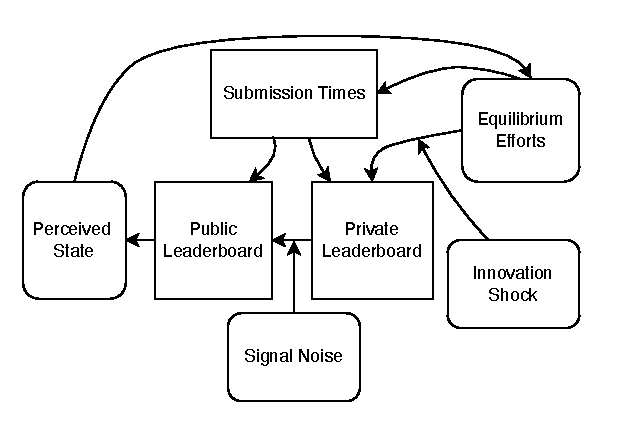
\includegraphics[scale=1.2]{kaggledata_diagram_simplified.pdf}
	\caption{Structure of a Typical Kaggle Contest}
	\label{kaggledata-diagram-simplified}
	\begin{minipage}{\textwidth}
{\footnotesize
\medskip
\textit{Note:} (1) Rectangles and rounded rectangles represent observed data and latent states, respectively. 
(2) The private leaderboard is visible only to the contest organizer during the contest and is revealed to all participants only after it ends.
During the contest period, contestants can observe only the submission times of each player and the public leaderboard.
}
\end{minipage}
\end{figure}


% Framework
To illustrate the framework in greater detail, Figure~\ref{kaggledata-diagram-simplified} depicts the key components and their interactions in a typical Kaggle contest.
% leaderboard
One notable feature is the existence of two leaderboards: a \textit{private} leaderboard, which is hidden until the contest ends and ultimately determines the final ranking and prize allocation, and a \textit{public} leaderboard, which is visible to all participants during the contest.\footnote{
This design serves two purposes. 
First, the public leaderboard provides participants with real-time feedback. 
Second, by keeping the private leaderboard concealed, the platform discourages overfitting to the public metric and preserves uncertainty, thereby sustaining competitive tension throughout the contest.
}
% submission
Both leaderboards are updated upon each submission.
% bayesian update
After observing the public leaderboard, contestants update their beliefs and form a perceived state of the competition.
% effort
Based on this belief, they choose their effort level, which corresponds to a \textit{Markov Perfect Equilibrium} (MPE).
% submission
These effort levels determine the submission intensity, and each submission triggers updates to both leaderboards.
% uncertainty
The private leaderboard, in particular, evolves according to the real-time effort level and an innovation shock.


% Structural estimation
We estimate the structural parameters of the model using a Bayesian approach, based on players’ submission times and the observed \textit{public} leaderboard trajectories from the Meta-Kaggle database.
% data
The estimation relies solely on information available to participants during the contest and leverages the equilibrium structure implied by the dynamic model.
% posteriors
This procedure enables us to recover a range of latent components that are not directly observable in the data, including the perceived state of the competition, the evolution of effort over time, individual ability levels, innovation uncertainty, and the precision of public signals.


% Cross-validation
To assess whether the estimated model captures the underlying structure of real-world contests, we perform a cross-validation exercise using out-of-sample data from the \textit{private} leaderboard.
As illustrated in Figure~\ref{kaggledata-diagram-simplified}, the volatility of the private leaderboard reflects the level of innovation risk in each contest, while the discrepancy between the private and public leaderboards captures the precision of the observed signal.
We estimate these contest-specific parameters independently and compare them against the corresponding values inferred from the Bayesian structural model.


% Results
Empirically, we carefully select 75 high-quality contests from the Meta-Kaggle database and preprocess the data to ensure consistency across estimation methods.
For each contest, we obtain two sets of contest-specific parameters—innovation risk and signal precision—using (i) our Bayesian structural estimation and (ii) a reduced-form approach based on private leaderboard dynamics.
We then perform regression analysis to compare the results from the two methods.
The findings reveal a strong and significant positive correlation between the two sets of estimates, validating the model’s ability to recover key latent elements that govern players’ strategic behaviour.


% Contributions
This paper makes two main contributions.
% 1. model
First, we develop a dynamic game-theoretic model and a Bayesian structural estimation framework, both tailored to real-world online crowdsourcing contests.
The model captures participants’ effort adjustments in response to evolving feedback and strategic interactions, and admits a tractable Markov Perfect Equilibrium underlying the structural estimation.
Together, they offer a parsimonious yet expressive framework for analyzing strategic behaviour in dynamic contest environments.
% 2. estimation
Second, we propose a cross-validation strategy that leverages out-of-sample data—specifically, the private leaderboard—which is naturally excluded from estimation yet reflects the same latent process modelled by the structure.
This design enables a direct and credible evaluation of whether the estimated structure captures key contest dynamics.
The results affirm the empirical relevance of the model and highlight its potential for mechanism evaluation and platform design.
Taken together, these contributions advance our understanding of online competitive dynamics and lay the groundwork for future empirical and policy applications.



\subsection{Related Literature}

This study is closely related to the below strands of literature:

\subsubsection{Contest Design.}

%% Static Contest Design
% definition
A rich literature on \textit{static} contest design \citep{ales2017optimal_award} investigates how to structure competitive environments to elicit optimal performance. 
These models typically rely on an explicit contest success function (CSF) that maps individual effort to winning probabilities \citep{skaperdas1996contest}.\footnote{There are exceptions like beauty or barrier contests.} 
Early contributions include \citet{Tullock1980}, \citet{Lazear1981tournaments}, and \citet{nalebuff1983Competition}. 
% application
This line of research is motivated by a wide range of real-world applications, including CEO selection \citep{tsoulouhas2006ceo}, beauty contests \citep{morris2002social}, election campaigns \citep{denter2020campaign}, advertising \citep{dockner2018Advertising}, litigation \citep{baik2007litigation, park2022litigation}, and innovation tournaments \citep{chen2021DataSharing}.
% design
Key design dimensions studied in the literature include optimal prize allocation \citep{moldovanu2001optimal, ales2017optimal_award}, participation rules \citep{ales2021number_of_players, stouras2022role}, contest duration\footnote{Static model in the sense that homogeneous participants make a single submission at the contest deadline, with no intermediate feedback provided throughout the process.} \citep{korpeoglu2021duration}, ex-ante handicapping of heterogeneous agents \citep{tsoulouhas2006ceo, kirkegaard2012favoritism, syam2013sales}, mechanisms addressing ex-post outcome imbalances \citep{Imhof2016Ex_post}, and information disclosure in auction-like environments \citep{bergemann2022optimal, antsygina2023optimal}. 


%% Dynamic Contest Design
% Transition
While these studies offer valuable insights into incentive design, they largely overlook how participants dynamically adjust their efforts in response to evolving competition.
% Dynamic Contest
In contrast, this paper focuses on \textit{dynamic} contests, where strategic decisions unfold over time.
Two main modeling approaches have been used to capture such dynamic strategic interactions:

% One Way: Poisson Arrival of Innovation Success
One strand of the literature models dynamic contests as multistage processes, where participants exert effort over time while facing uncertainty about intermediate progress.
This structure facilitates the analysis of the mid-contest policy instruments available to the contest designer, such as feedback disclosure, screening mechanisms, etc.
Specifically, in a typical two-stage setting \citep{aoyagi2010information, mihm2019feedback}, the initial stage captures either feasibility uncertainty or foundational experimentation, with progress revealed through milestone feedback provided by the contest organizer. 
Participants exert effort in both stages, and the final output reflects the cumulative impact of early performance and subsequent improvement.
Similarly, \citet{bimpikis2019designing} study a two-stage model in which agents exert continuous effort to complete Stage A (potentially infeasible) and Stage B (feasible), with breakthroughs governed by Poisson processes.
In all these models, the contest designer may strategically disclose interim feedback.
Another example is \citet{Khorasani2023screening}, who analyze a two-stage contest in which solvers invest exploratory effort to generate viable ideas, with only those passing an imperfect screening mechanism proceeding to execution.

% Another Way of Modelling
The second approach, more closely related to our work, treats output as a stochastic process whose drift depends on the participant’s effort.
This line of research originates from the tug-of-war framework, first formalized by \citet{Harris1987Race} as a one-dimensional simplification of a multi-stage R\&D race.
Subsequent studies build on this foundation by modeling each player’s progress as a Brownian motion.
\citet{budd1993Duopoly}, for example, analyze a duopoly innovation race where the state evolves as a Brownian motion driven by the difference in effort, and characterize an approximate equilibrium.
\citet{Moscarini2007Contest} advance this approach by modeling the game state as the output gap between players and derive closed-form equilibrium strategies under pure-strategy play.
\citet{Ryvkin2022Fight} adapt their framework to a dynamic contest with a fixed deadline, providing a closed-form solution for the Markov perfect equilibrium.


%% Online Crowdsourcing
% this paper
This paper studies online crowdsourcing contests, which are typically characterized by 
$i$) fixed deadlines, 
$ii$) repeated submissions, and 
$iii$) public real-time feedback,
all governed by platform-specific rules and evaluation metrics.
% our foundation
Hence, our analysis builds on the model by \citet{Ryvkin2022Fight}, which, despite its simplifications, offers a closed-form solution that balances realism with analytical tractability. 
To better reflect the dynamics of online leaderboards, we depart from their full-information setting by introducing a noisy real-time public signal, thereby enhancing the model’s empirical relevance.



\subsubsection{Structural Estimation of Contests.}

Beyond theoretical modelling, a growing body of research employs structural estimation techniques to recover key parameters of contest environments using observed data.

% Static contests
In the structural estimation of static contests, when a contest success function (CSF) is explicitly specified, the primary goal is to estimate its functional form or key parameters \citep{hwang2012technology, kang2016policy, huang2021structural}.
In contrast, for contests without a well-defined or smooth CSF—such as beauty contests—researchers typically rely on equilibrium conditions, most notably the first-order condition.
For example, \citet{yoganarasimhan2016estimation} proposes a two-step semiparametric estimator, resembling the EM algorithm, to recover both unobserved auction heterogeneity and bidder cost distributions.
Similarly, in auction-like models \citep{guerre2000optimal, shakhgildyan2022nonparametric}, nonparametric estimation of the underlying valuation structure often serves as a first step, providing the foundation for subsequent structural estimation.

% Dynamic contests
Most dynamic structural estimations rely on the Markov Perfect Equilibrium (MPE) of a dynamic game. 
However, when the model is calibrated to closely fit real-world data, the MPE typically lacks a closed-form solution.
For example, \citet{jiang2022feedback} develop a finite-horizon dynamic game with discrete time, state, and action spaces to model creators’ strategic behaviour in response to feedback during online logo design contests.
Using data from 810 contests, they implement a two-step maximum likelihood estimation (MLE) procedure under the assumption of ex-ante homogeneous contests and players: the first step estimates action-specific state transition probabilities, while the second recovers utility parameters.

Specific to online crowdsourcing environments, 
\citet{chen2021attracting} use data from 1,980 contests on TaskCN.com to examine how contest duration affects both the number and quality of participants.
Through regression analysis, they show that while longer durations attract more contestants, they tend to reduce the quality of top entrants.
\citet{zhang2019structural} build a dynamic structural model to study how participants in crowdsourcing contests learn and choose contests over time.
Their model shows that competing against superstars accelerates learning by providing more informative feedback.
Using Bayesian updating and a hierarchical model, they estimate how individuals trade off monetary rewards, learning opportunities, and participation costs, based on data from Topcoder.

Closely related to our work, \citet{lemus2021dynamic} conduct contest-level structural estimation using Kaggle data.
They propose a finite-horizon dynamic game in which, after each submission, players decide whether to continue or exit, essentially solving an optimal stopping problem.
Players can only make this decision immediately after completing a submission, which arrives at random intervals and incurs a privately drawn cost.
Their estimation proceeds in two stages: the first uses maximum likelihood and the EM algorithm to estimate primitive parameters such as the distribution of player types and scores; the second applies a CCP-based estimator to identify the cost distribution.
Our model differs in two key respects: 
(1) we treat submissions as the outcome of accumulative effort rather than discrete costly actions—an assumption that better reflects actual player behaviour; and
(2) we explicitly model belief updating from signals to identify structural parameters, whereas their CCP-based method relies on a coarser behavioural approximation.







The structure of the paper is as follows: 
Section~\ref{contest-theory} introduces our theoretical model of online crowdsourcing contests. 
Section~\ref{sect-bayes-framework} presents the Bayesian estimation framework. 
In Section~\ref{sect-synthetic}, we describe the data-generating process and apply the Bayesian framework to synthetic data. 
Section~\ref{sec-kaggle-application} validates the theoretical model using real-world data. 
All code and implementation details are available on GitHub.



\section{The Model}\label{contest-theory}

% Effort, Output and Gap
Two players, $i$ and $j$, compete for a prize $\theta>0$ in a contest. 
Winner gets the prize and loser gets nothing. 
The contest starts at time zero. 
At every time $t\ge0$, the representative player $i$ chooses an effort level $q_{i,t}$ and burdens a quadratic cost $C_i(q_{i,t}) = c_i q_{i,t}^2/2$, with a lower $c_i$ corresponding to higher ability. 
Denoted by $y_t$ the \textit{output gap} of player $i$ and $j$ at time $t$, driven by
\begin{equation}\label{eq-state-dynamics}
	dy_t = (q_{i,t}-q_{j,t})dt + \sigma dW_t
\end{equation}
where $W_t$ is a Brownian motion and $\sigma>0$ measures the innovation risk.
When $\sigma$ is large and the relationship between effort and output is highly uncertain, luck becomes the dominant factor. 
Conversely, when $\sigma$ is small and output closely reflects effort, the importance of effort is amplified.

The contest is equipped with a submission system that allows participants to upload their algorithms at any time and receive immediate feedback. 
For simplicity, we further assume that agents submit their intermediate results whenever they make progress. 
This setup enables the contest organizers to monitor all players’ progress $x_{i,t}$ and $x_{j,t}$ in real time. 
Moreover, the true output level, evaluated by the system, is only known by the game designer but not the two players. 
% Signal
At any time $t>0$, the contest designer emits a \textit{public} signal of the real output gap $y_t$. 
The signal is ambiguous and the game holder controls the ambiguity. 
The dynamic of signal is  
\begin{equation}\label{signal}
	dZ_{t} = y_{t}dt + \frac{dB_{t}}{\sqrt{\lambda}} 
\end{equation}
where $B_{t}$ is standard Brownian motion independent with $(W_{i,t})$ and $(W_{j,t})$, and the parameter $\lambda$ is set by the game holder to control the precision of signal. 
A larger $\lambda$ implies less noise in the signal, enhancing its reliability; conversely, a smaller $\lambda$ indicates greater noise, making the signal less trustworthy. 

% Bayesian Player
The information set of both players at time $t \ge 0$ is  $I_{t} \equiv \{Z_{s} : 0\le s \le t\}$. 
Player $i$ estimates the unknown output gap $y_t$ based on the information set $I_t$. 
Let $\tilde{y}_t \equiv E(y_{t}|I_t)$ be the estimated output gap and $S_t \equiv E[(\tilde{y}_{t}-y_{t})^2|I_t]$ be the estimation variance. 
According to Chapter 1.2 of \citet{Bensoussan1992Control}, \textit{Kalman-Bucy filter} (See related discussions in \citealt{frogerais2012various}, \citealt{barrau2017invariant}) gives the dynamics of $\tilde{y}_{t}$ and $S_{t}$, 
\begin{align}
	d\tilde{y}_{t} &= (q_{i,t}-q_{j,t})dt + \lambda S_{t}(dZ_{t}-\tilde{y}_{t}dt) 
	\label{filtered-x}\\
	\frac{dS_{t}}{dt} &= \sigma^2 - \lambda S_{t}^2
	\label{filtered-S}
\end{align} 
Hence, the conditional distribution $y_{t}|I_t\sim\mathcal{N}(\tilde{y}_{t},S_{t}|I_t)$ is fully captured by the mean $\tilde{y}_{t}$ and variance $S_{t}$. 
If $\lambda = 0$, we have $S_t = S_0+\sigma^2t$, i.e., the estimation variance is increasing in time linearly. 
If $\lambda > 0$, the solution of (\ref{filtered-S}) is
\begin{equation}\label{S-evolution} 
	S_t = 
	\begin{cases}
        \bar{S} \cdot \tanh\left\{t\cdot\sigma\sqrt{\lambda} +  \tanh^{-1}\left(S_0\big/\bar{S}\right)\right\} & \text{if } S_0 < \bar{S} \\
        \bar{S} & \text{if } S_0 = \bar{S} \\
        \bar{S} \cdot \coth\left\{t\cdot\sigma\sqrt{\lambda} +  \coth^{-1}\left(S_0\big/\bar{S}\right)\right\} & \text{if } S_0 > \bar{S} 
	\end{cases}
\end{equation}
Specifically, $\bar{S} = \sigma / \sqrt{\lambda}$ when $\lambda>0$ and $\bar{S} = \infty$ when $\lambda = 0$. 
Please refer to Appendix~\ref{app-S-equ} for the derivations. 
In Figure~\ref{fig-S-evol}, we show the evolution of $S_t$ in time: estimation variance $S_t$ converges to \textit{steady state} $\bar{S}$ as time goes by regardless of the starting estimation variance. 
For simplicity, we henceforth assume that $S_0 = \bar{S}$, hence $S_t\equiv \bar{S}$. 

\begin{figure}[!ht]
	\centering
	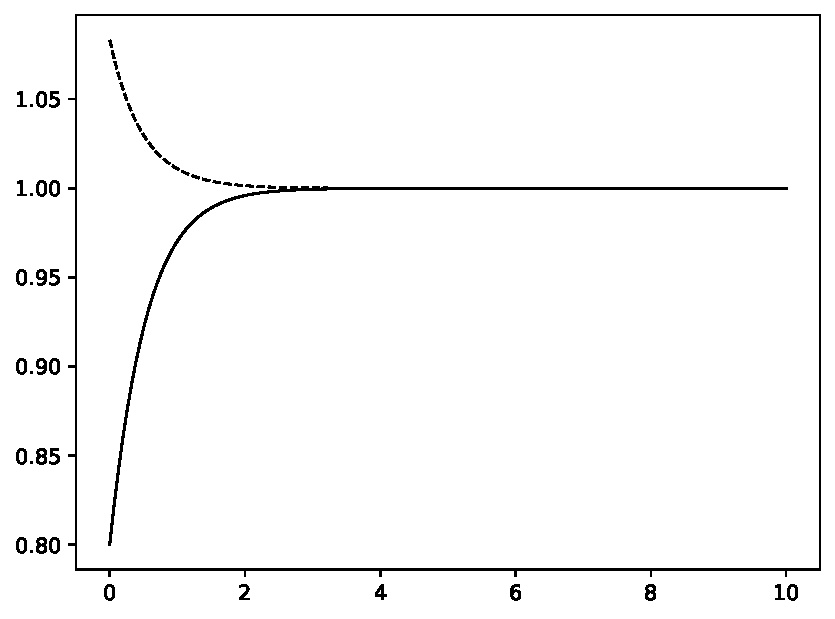
\includegraphics[scale=0.6]{figure_S_evolve.pdf}
	\caption{The evolution of $S_t$ in time $t$, given that $\lambda = 1$ and $\sigma = 1$.} \label{fig-S-evol}
\end{figure}



% Contest Deadline
Following \cite{Ryvkin2022Fight}, let's consider a dynamic contest with a fixed deadline. 
Suppose the contest is terminated when time $t=T>0$. 
Since the steady state estimation variance $\bar{S}$ is fixed as displayed above, the state of the game is fully characterized by a tuple $(\tilde{y}_t, t)$. 
At any time $0\le t<T$, player $i$ optimizes her effort level $q_{i,\tau}$ in the remaining contest period $\tau\in[t, T)$ according to the following optimization problem, 
\begin{equation}\label{v-def}
	V^i(\tilde{y}_{t}, t ; q_{j,t},\Theta_i) = \max_{\{q_{i,\tau}\}^T_{\tau=t}} 
	\mathbb{E}\left( \theta\cdot1_{\tilde{y}_T>0} - \int^T_tC_i(q_{i,\tau})d\tau \bigg|I_t\right) 
\end{equation}
where $\Theta_i \equiv\{\theta, \lambda, \sigma, c_i\}$, subject to constraints (\ref{filtered-x}), (\ref{filtered-S}) and $q_{i,\tau}\ge0$ for all $\tau\in[t,T)$.
The optimization problem for player $j$ is just symmetric to that of player $i$ as $V^j(\tilde{y}_t, t) = V^i(-\tilde{y}_t, t)$. 
The corresponding Hamilton-Jacobi-Bellman (HJB) equation for player $i$ is 
\begin{equation*}
0 = \max_{q_{i,t}\ge0}\left[-\frac{c_iq_i^2}{2} + V^i_{y}\cdot\left(q_{i,t}-q_{j,t}\right)+V^i_t + \frac{V^i_{yy}}{2}\lambda \bar{S}^2\right].
\end{equation*}
By definition, we have $\lambda \bar{S}^2 = \sigma^2$. 
Under the assumption of inner solution, we plug into the first order conditions $q_{i,t} = V^i_y/c_i$ and $q_{j,t} = -V^j_y/c_j$, we have the system of equations
\begin{equation*}
\begin{aligned}
\frac{1}{2c_i}(V^i_y)^2 + \frac{1}{c_j}V^i_yV^j_y + V^i_t + V^i_{yy}\frac{\sigma^2}{2} = 0\\
\frac{1}{2c_j}(V^j_y)^2 + \frac{1}{c_i}V^j_yV^i_y + V^j_t + V^j_{yy}\frac{\sigma^2}{2} = 0
\end{aligned}
\end{equation*}
subject to boundary conditions $V^i(-\infty, t) = 0$, $V^i(+\infty, t) = \theta$, $V^j(-\infty, t) = \theta$, $V^j(+\infty, t)=0$, $V^i(\tilde{y}_T, T) = \theta \cdot 1_{\tilde{y}_T > 0}$ and $V^j(\tilde{y}_T, T) = \theta \cdot 1_{\tilde{y}_T < 0}$. 


The Nash equilibrium is summarized in the following lemma. 
We include a simplified version of the proof in the appendix: 

\begin{theorem}[\citealt{Ryvkin2022Fight}]
In the Markov perfect equilibrium, the players’ efforts in state $m_{i(j)}(\tilde{y}_t, t) :\mathbb{R}\times[0, T)\to\mathbb{R}_+$ are given by
\begin{equation}\label{eq-equilibrium-effort}
m_{i(j)}(\tilde{y}_t, t) = \frac{e^{-z^2/2}}{\sqrt{2\pi\sigma^2(T-t)}}\cdot \frac{\sigma^2}{2}\left[\gamma(\rho_{i}) + \gamma(\rho_{j})\right]\left[1-\rho(z)^2\right]\left[1 \pm \rho(z)\right]
\end{equation}
where $z = \tilde{y}_t / (\sigma\sqrt{T-t})$, $\rho(z) = \gamma^{-1}\left(\Phi(z)\left[\gamma(\rho_{i})+\gamma(\rho_{j})\right]-\gamma(\rho_{j})\right)$ and 
\begin{equation*}
\gamma(u) = \frac{u}{1-u^2} + \frac{1}{2}\ln\frac{1+u}{1-u},\quad u\in(-1,1)
\end{equation*}
\begin{equation*}
\rho_{i} = \frac{e^{w_{i}}+e^{-w_{j}}-2}{e^{w_{i}}-e^{-w_{j}}},
\quad
\rho_{j} = \frac{e^{w_{j}}+e^{-w_{i}}-2}{e^{w_{j}}-e^{-w_{i}}},
\quad
w_{i(j)} = \frac{\theta}{\sigma^2 c_{i(j)}}.
\end{equation*}
Moreover, the total expected effort at time $t$, defined by $M(\tilde{y}_t, t) := \mathbb{E}\left[\int^T_t m_i(\tilde{y}_s, s) + m_j(\tilde{y}_s, s)ds\right]$, is given by $M(\tilde{y}_t, t) = \sigma \sqrt{T-t} q(z)$, where $q(z)$ is determined by the ordanary differential equation 
\begin{equation}
\begin{aligned}
&q''(z) + \left[4A_+(z)e^{-z^2/2}+z\right]q'(z) - q(z) + 4A_-(z)e^{-z^2/2} = 0\\
&A_-(z) = \frac{\gamma(\rho_1) + \gamma(\rho_2)}{2\sqrt{2\pi}}[1 - \rho(z)^2],
\quad A_+(z) = A_-(z)\rho(z)
\end{aligned}
\end{equation}
subject to the boundary conditions $q(z)\to0$ as $z\to\pm\infty$. 
Specifically, when $c_i = c_j$, we have $w_i = w_j = w$ and the total expected effort is reduced to 
\begin{equation}\label{eq-totaleffort-reduced}
M(\tilde{y}_t, t) = \frac{2w\sigma\sqrt{T-t}}{\sqrt{2\pi}}e^{-z^2/2} + o(w)
\end{equation}
\end{theorem}

\begin{remark}
The value of $w$ is sufficiently small when the uncertainty level $\sigma$ is sufficiently large compared to prize-cost ratio $\theta/c_{i(j)}$. 
\end{remark}

In equation (\ref{eq-equilibrium-effort}), the variables $w_{i(j)}$ measure the abilities of two players, while $\rho_{i(j)}$ normalizes $w_{i(j)}$ into the interval $(0, 1)$. 
Specifically, $\rho_{i(k)}$ and $w_{i(j)}$ are in a strictly increasing bijective relationship. 
It is not hard to see that function $\gamma(\cdot)$ is strictly increasing on $(-1,1)$, ranging from $-\infty$ to $+\infty$. 
The function $\rho(\cdot)$ is strictly increasing on $\mathbb{R}$, ranging from $-1$ to $1$. 
%% Forms
The equilibrium effort $m_{i(j)}$ can be represented to the product of two components:
the normal density function $\phi(y; 0, \sigma^2(T-t))$, which represents the probability density of a normal distribution with mean zero and variance $\sigma^2(T-t)$ evaluated at state $y$, and an amplitude factor $K_{i(j)}(z; \theta, \sigma, c_i, c_j) := \frac{\sigma^2}{2}\left[\gamma(\rho_{i}) + \gamma(\rho_{j})\right]\left[1-\rho(z)^2\right]\left[1 \pm \rho(z)\right]$. 
The normal density governs the concentration of competitive intensity over state, i.e., perceived output gap $\tilde{y}_t$, while the amplitude term $K_{i(j)}$ modulates the asymmetry (or skewness) of effort allocation between players.

It is also evident that the parameters $\theta$, $c_i$ and $c_j$ influence equilibrium effort exclusively through the amplitude component.
In contrast, the effect of $\sigma$ is more nuanced, as it enters both the normal density and amplitude terms. 
Based on the structure of (\ref{eq-equilibrium-effort}), we further conclude that the equilibrium effort level is \textit{not} uniformly increasing in the prize-cost ratio $\theta/c_{i(j)}$ across all states $\tilde{y}$—particularly for laggard states.
The uncertainty term $\sigma$ and the remaining time $T - t$ make the equilibrium effort more dispersed: under high uncertainty or with ample remaining time, players exert higher effort in extreme states and lower effort in central states.
As time progresses and the deadline approaches, outcomes become more predictable, and effort becomes increasingly concentrated around the pivot state.

For more properties of the equilibrium, please refer to \citet{Ryvkin2022Fight}. 
Here, we only provide a supplementary analysis related to contest design:


\subsection{Implications on the Contest Design}

In online crowdsourcing contests, designers typically control key decision variables such as the prize amount $\theta$ (we exclude more complex prize structures in this study), the contest duration $T$, and the signal precision $\lambda$. 
A key concern is that these variables may act as substitutes—implying that the optimal choice of one may alter or offset the optimal choices of the others.

A first observation is that the signal precision $\lambda$ does not influence the total expected effort $M(\tilde{y}_t, t)$.
Under the simplifying assumption that $S_t = \bar{S}$ is constant, the incorporation of signals does not reduce overall uncertainty.
As a result, the evolution of the filtered state $\tilde{y}_t$ in (\ref{filtered-x}) does not lead to an increase in $M(\tilde{y}_t, t)$ compared to the unfiltered state $y_t$ specified in (\ref{eq-state-dynamics}).\footnote{
However, this result primarily reflects the limitations of our model.
In a more general setting with fewer restrictions, the signal precision parameter $\lambda$ would clearly affect the structure of $M$,
although such cases are beyond the scope of this paper.
}

Next, we turn to the other two design variables.
When the two contestants are of similar strength, i.e., $c_i = c_j = c$, the total expected effort admits a particularly simple approximation, as shown in equation (\ref{eq-totaleffort-reduced}).
Suppose the contest designer’s objective takes the form $\beta^{T}M(\tilde{y}_0, 0)^\alpha - \theta$ for some $0 < \alpha < 1$ and $0 < \beta \le 1$,
it is straightforward to show that this objective function is jointly concave in $(\theta, T)$.




\section{Estimation Framework}\label{sect-bayes-framework}

In this section, we describe the estimation procedure. 
We first outline the data generation process, establishing the connection between the empirical data and the theoretical model discussed previously.
Then, we introduce a structural estimation method using Bayesian framework.

\subsection{Data-Generating Process}

For each Kaggle contest, the observable data from the Meta-Kaggle dataset can be categorized into three main components:

%% Data: Contest setting
The first component consists of essential contest details, including the contest duration, prize structure, information disclosure policy, and other governing rules.
%%%% Prob 1
Contrary to the assumptions of our model, a typical contest usually involves multiple teams rather than just two.
In Section~\ref{sec-kaggle-application}, we focus on the two strongest participants in each contest for analysis.
%%%% Prob 2
Furthermore, many contests adopt complex prize structures, offering multiple awards rather than following a winner-takes-all format.
In Section~\ref{sec-kaggle-application}, we begin by selecting contests that offer a single prize awarded in USD.

%% Data: Submissions
The second component captures the submission events of each player $i$ to the system, denoted by the sequence $\{\hat{t}^i_k\}_{k=1}^{N_i}$.
Here, $N_i$ represents for the total number of submissions by player $i$, and $t$ represents for the time of each submission. 
We understand the submission events of player $i$ and $j$ as two conditional independent inhomogeneous Poisson processes, driven by the intensity functions $\tau_i(t)$ and $\tau_j(t)$.\footnote{That is, given the intensity functions $\tau_i(t)$ and $\tau_j(t)$, the submission events $\{\hat{t}^i_k\}_{k=1}^{N_i}$ and $\{\hat{t}^j_k\}_{k=1}^{N_i}$ are mutually independent.}
Then, during any time interval $\mathcal{S}$ of the contest duration $\mathcal{T}$, the Poisson arrival rate of submissions of the representative player $i$ is given by $\int_{s\in\mathcal{S}}\tau_i(s)ds$. 
We assume the submission intensity $\tau_i(t)$ is proportional to the effort level $m_i(\tilde{y}_t, t)$. More specifically, 
\begin{equation}\label{eq-model-intensity}
\tau_i(t) = r \cdot m_i(\tilde{y}_t, t)
\end{equation}
where $r>0$ is the ratio of submission intensity to effort level, serving as a tuning parameter for numerical stability. 


%% Data: Leaderboard
The third component of the contest data is the \textit{public} and \textit{private} leaderboard that records the real-time rankings and scores of each participant, denoted by $\hat{x}^{i(j)}_t$ and $x^{i(j)}_t$. 
In Kaggle competitions, most organizers deliberately disclose only a subset of the full dataset to participants to mitigate the risk of overfitting. 
The proportion of the released data is generally known to all participants. 
The public leaderboard is updated upon each submission, using only the released portion of the dataset; as a result, the signals it provides are inherently noisy.
In addition to the public leaderboard, most competitions hosted on Kaggle also maintain a private leaderboard, where organizers evaluate the true predictive performance of participants’ models using the full dataset.
The true output gap $y_t := x^i_t - x^j_t$ is generated according to equation (\ref{eq-state-dynamics}).
It is observable only by the game designer during the contest and becomes available from the Meta-Kaggle dataset after the contest concludes. 
Furthermore, we interpret the difference in scores between $i$ and $j$ displayed on the public leaderboard as the signal $Z_t$ defined in (\ref{signal}), released by the contest organizer. 
Specifically, let's denote $\hat{y}_t = \hat{x}^i_t - \hat{x}^j_t$ the gap between displayed scores, and interpret it as the signal intentionally released by the contest organizer: 
\begin{equation}\label{eq-model-signal}
dZ_t = \hat{y}_tdt
\end{equation}
Combining (\ref{signal}) with (\ref{eq-state-dynamics}), the observed real-time gap $\hat{y}_t$ on leaderboard evolves as 
\begin{equation}\label{eq-leaderboard-gap}
\hat{y}_t = y_t + \frac{1}{\sqrt{\lambda}}\frac{dB_t}{dt} = \int^t_0\left[m_i(\tilde{y}_t, s) - m_j(\tilde{y}_t, s)\right]ds + \sigma W_{t} + \frac{\xi_t}{\sqrt{\lambda}}
\end{equation}
where the term $\sigma W_t$ captures the accumulated innovation shock, $\lambda$ governs the signal precision and $\xi_t$ is a white noise with $\mathbb{E}(\xi_t\xi_s) = \delta(t-s)$. 
In practise, we approximately assume that $\xi_t \approx (B_{t+\Delta} - B_t)/\Delta$ where $\Delta$ is a small time interval. 

% tilde{y}_t
It is important to recognize that the generation of $y_t$ and $\hat{y}_t$ is inherently tied to the players’ strategic interactions, as it depends on their estimates of the underlying state, $\tilde{y}_t$. 
In turn, $\tilde{y}_t$ evolves dynamically based on $\hat{y}_t$, since players continually update their beliefs in response to observed data. 
As a result, the generation of $y_t$, $\hat{y}_t$ and $\tilde{y}_t$ proceeds jointly.
By equations (\ref{filtered-x}) and (\ref{eq-model-signal}), the estimated gap $\tilde{y}_t$ as perceived by the two players, is determined by the following stochastic differential equation:
\begin{equation}\label{eq-fintered-y-update}
d\tilde{y}_{t} = \left[m_i(\tilde{y}_t, t) - m_j(\tilde{y}_t, t)\right]dt + \sqrt{\lambda}\sigma(\hat{y}_t-\tilde{y}_{t}) dt
\end{equation}
with initial condition $\tilde{y}_0 = \mu_0$, where $\mu_0$ can be interpreted as the prior mean of the initial true state $y_0$.

We denote the set of unknown parameters by $\Theta := \{c_i, c_j, \sigma, \lambda, \mu_0\}$.
Once $\Theta$ is specified, the data-generating processes for $(y_t)$, $(\hat{y}_t)$, and $(\tilde{y}_t)$ are fully defined by equations (\ref{eq-state-dynamics}), (\ref{eq-leaderboard-gap}), and (\ref{eq-fintered-y-update}), although their realized trajectories remain stochastic.



\subsection{Discussions}

\subsubsection{Strategic submission timing.}

Beyond the uncertainty caused by partial data disclosure, an additional source of signal noise stems from the timing of leaderboard updates: rankings are only refreshed upon new submissions, rendering the leaderboard uninformative during periods of inactivity.
This lag would significantly bias model estimates if participants deliberately timed their submissions. 


In our data-generating process, however, we assume that submissions are entirely driven by effort and do not explicitly model strategic timing behaviour, thereby abstracting away from this issue.
Strategic submission timing is, in fact, a well-known concern in the literature. 
For example, \citet{lemus2021dynamic} adopt a similar simplification by excluding such behavior from their model.
As a partial remedy in our empirical design, we require a minimum number of submissions when selecting the two representative players (see Section~\ref{sec-data-clean}).
This helps reduce the likelihood of manipulation—such as intentionally delaying or withholding submissions to mislead competitors.


\subsubsection{Selection of Two Players.}

An additional concern underlying the data-generating process pertains to the assumption that there are only two contestants participating in the entire competition.
The implication of this assumption in the context of crowdsourcing platforms like Kaggle is that each team has a clear understanding of the capabilities of all other competitors, allowing the two strongest teams to mutually recognize each other. 
In reality, however, this assumption considerably oversimplifies the problem.
In Section~\ref{sect-robust-2players}, we conduct a series of robustness checks. 
By selecting the top two competitors using alternative criteria, we aim to assess whether the earlier conclusions remain valid.

\subsubsection{Normality.}

Another aspect of the data-generating assumptions that may be open to question is the assumption of normality. 
Specifically, we rely on normal distributions in two critical components: the signal noise and the innovation shock. 
As discussed in Section~\ref{sec-data-clean}, maintaining this assumption depends heavily on our data transformation procedures, such as converting percentage leaderboard data into the state variable $\hat{y}_t$. 
When applying a uniform transformation across all contests, we find that for many contests, approximately half, the resulting data do not conform well to a normal distribution. 
This discrepancy has important implications for the credibility of our statistical results.
In Section~\ref{sect-robust-normality}, we adopt alternative data processing methods to assess the robustness of our results.



\subsection{Bayesian Estimation Framework}

Our objective is to develop a Bayesian framework for inferring the unknown parameter set $\Theta := \{ c_i, c_j, \sigma, \lambda, \mu_0 \}$ using the data introduced above.

First of all, we assume that time is discretized into uniform intervals of length $\Delta$.
By definition, the likelihood function corresponding to the submission times of player $i$, $\{t^i_k\}_{k=1}^{N_i}$, is given as follows (a symmetric formulation applies to player $j$):
\begin{equation}\label{eq-ihpp-prob}
p\left(\{\hat{t}^i_k\}_{k=1}^{N_i} | \tau_i, \Theta\right) = \exp\left\{-\int_{s\in\mathcal{T}}\tau_i(s)ds\right\}\prod_{k=1}^{N_i}\tau_i(\hat{t}^i_k)
\end{equation}
where $\tau_i$ is defined in (\ref{eq-model-intensity}) with the tuning parameter $r$ exogenously specified. 
Since time is discretized, the integrals on the left-hand side can be approximated by finite sums.

Next, suppose the public leaderboard gaps $\hat{y}_t$ is sampled at time points $(t_1, t_2, ..., t_N)$, yielding observations $\{\hat{y}_{t_k}\}^N_{k=1}$. 
Let $t_0 = 0$ and suppose the initial gap satisfies $y_0 = 0$. 
Then, according to the assumed data-generating process of $\hat{y}_t$ in (\ref{eq-leaderboard-gap}), the corresponding likelihood function is
\begin{equation}\label{eq-obs_gap-prob}
p\left(\{\hat{y}_{t_k}\}_{k=1}^N | \{\hat{t}^{i(j)}_k\}_{k=1}^{N_{i(j)}}, m_i, m_j, \Theta\right) = 
\phi\left(\{\hat{y}_{t_k}\}_{k=1}^N | \left\{\mu_k\right\}^N_{k=1}, \Sigma_y+\frac{I_N}{\Delta\lambda}\right)
\end{equation}
where $\mu_k = \int_{0}^{t_{k}}m_i(\tilde{y}_s, s) - m_j(\tilde{y}_s, s)ds$ and $\Sigma_y(i, j) = \sigma^2\min(t_i,t_j)$. 
Moreover, let $N = N_i + N_j$, indicating that the public leaderboard is updated once a new submission occurs. 

%% Note: exclude y_t in likelihood
It's worthwhile noting that, although the trajectory of private leaderboard $y_t$ is available ex post from the Meta-Kaggle dataset, we deliberately exclude it from the likelihood function. 
In our framework, agents form beliefs about $y_t$ based solely on $\hat{y}_t$, and their actions are driven by these beliefs. 
Conditioning on the realized values of $y_t$ in estimation would effectively bypass the agent’s informational constraints and undermine the role of $\lambda$ in shaping belief formation. 
More importantly, it would prevent us from evaluating whether the proposed model—when given only the information actually available to agents—can recover the true data-generating process. 
Treating $y_t$ as latent therefore preserves the integrity of the causal structure and enables meaningful model validation after estimation (see Figure~\ref{kaggledata-diagram}).

%% Approximation
To evaluate the likelihood functions (\ref{eq-ihpp-prob}) and (\ref{eq-obs_gap-prob}), we must first compute the equilibrium trajectories of both the perceived output gap $(\tilde{y}_t)$ and the effort levels $(m_i(\tilde{y}_t, t), m_j(\tilde{y}_t, t))$, as implied by equations (\ref{eq-equilibrium-effort}) and (\ref{eq-fintered-y-update}). 
Importantly, the construction of $\tilde{y}$ and the effort functions $m_i$ and $m_j$ depends on the underlying (unobserved) parameters $c_i$, $c_j$, $\sigma$ and $\lambda$, which are themselves subject to estimation.

Once these parameters are specified, the equilibrium paths of the perceived output gap $(\tilde{y}_t)$ and the corresponding effort levels $(m_i(\tilde{y}_t, t), m_j(\tilde{y}_t, t))$ can be deterministically computed. 
However, evaluating $m_{i(j)}(\tilde{y}_t, t)$ via equation~(\ref{eq-equilibrium-effort}) requires numerically approximating the inverse function $\gamma^{-1}$, which poses challenges for the use of gradient-based Markov Chain Monte Carlo (MCMC) sampling methods, such as Hamiltonian Monte Carlo (HMC, \citealt{neal1996bayesian}, \citealt{neal2011mcmc}, \citealt{betancourt2017conceptual}) and the No-U-Turn Sampler (NUTS, \citealt{hoffman2014NUTS}).
Hence, we approximate this inverse function with an analytical form:
\begin{equation}\label{eq-invgamma-approx}
\gamma^{-1}(x) \approx \frac{2}{\pi}\arctan(a \cdot x)
\end{equation}
where $a$ is around 0.947 by minimizing the 1-norm of the difference between the numerical inverse of $\gamma(\cdot)$ and the approximation $\frac{2}{\pi} \arctan(a x).$\footnote{Under infinity norm, the parameter $a = 0.856$; under 2-norm, the parameter $a=0.895$.}
Figure~\ref{fig-approximation} compares the equilibrium effort function $m_i(\tilde{y}_t, t)$ derived from the approximate analytical form of $\gamma^{-1}$ in equation~(\ref{eq-invgamma-approx}) with that obtained from the numerically accurate solution.
As illustrated, the approximation closely replicates the true function.

\begin{figure}[!ht]
    \centering
    \begin{subfigure}{0.48\textwidth}
        \centering
        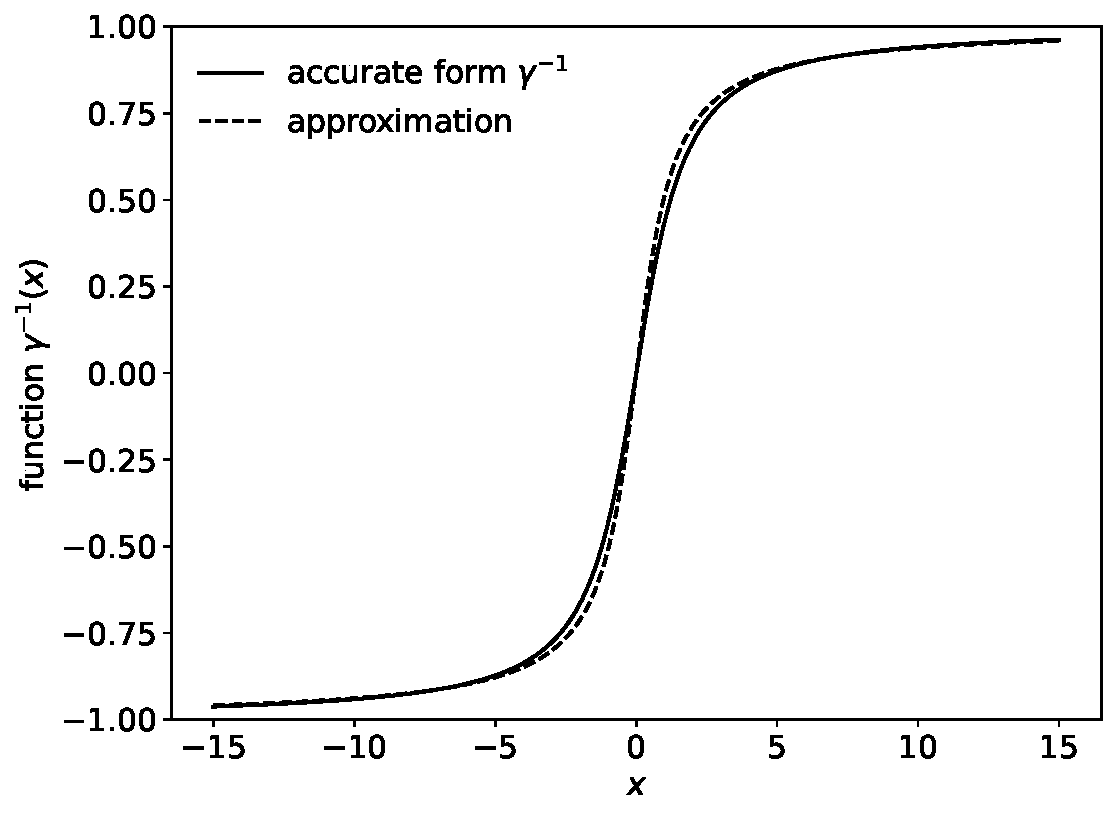
\includegraphics[width=\linewidth]{approx_invgamma.pdf}
        \caption{Auxiliary Function $\gamma^{-1}(x)$}
    \end{subfigure}
    \hfill
    \begin{subfigure}{0.48\textwidth}
        \centering
        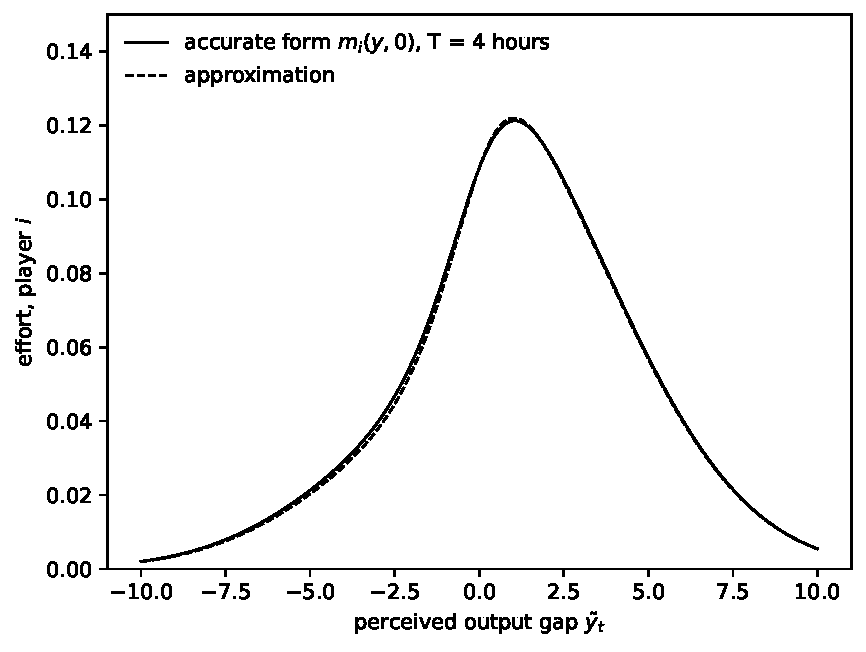
\includegraphics[width=\linewidth]{approx_equi_effort.pdf}
        \caption{Equilibrium Effort $m_i(\tilde{y}_t, t)$}
    \end{subfigure}
    \caption{Comparison of the Accurate and Approximate Forms ($\theta = 1$, $c_i = c_j = 1$, $\sigma=1$, $\Delta=1/24$)}
    \label{fig-approximation}
\end{figure}

In our Bayesian framework, we specify truncated normal distributions with large variances as priors for the unknown parameters $\Theta$.
This choice is intended to make the priors as uninformative as possible, thereby minimizing their influence on the posterior distribution. 
By allowing the parameters to vary broadly within reasonable bounds, these weakly informative priors let the data play a dominant role in shaping the inference, while still ensuring mathematical well-posedness and numerical stability.


The following lemma establishes the identifiability of the model parameters.

\begin{lemma}\label{lmm-params-identifiability}
The contest parameters $c_i$, $c_j$, $\sigma$, $\lambda$ and $\mu_0$ are jointly identifiable. 
\end{lemma}




\section{Synthetic Experiments}\label{sect-synthetic}

Before applying our estimation procedure to real-world contest data, we evaluate its potential on synthetically generated data. 
The use of synthetic data serves not only to validate the effectiveness of Bayesian inference, but also to enhance our understanding of the underlying data-generating process, which is summarized in Algorithm~\ref{algo-dgp}. 

\begin{algorithm}[!ht]
\caption{Synthetic Data Simulation}
\label{algo-dgp}
\begin{algorithmic}
\STATE \textbf{Input:} 
	$\Delta$, $T$, $c_i$, $c_j$, $\sigma$, $\lambda$, $r$, $\tau^\star$, $y_0$, $\mu_0$
\STATE Sample $\{s_k^{i(j)}\}^{N_{i(j)}}_{k=1}$ from Poisson process $(\tau^\star)$ on $[0, T)$
\STATE Sample $\{u_k^{i(j)}\}^{N_{i(j)}}_{k=1}$ from uniform distribution on $[0, 1]$
\STATE Sample series of Brownian motions $(W_t)$ and $(B_t)$
\STATE Initialize $\ell^{i(j)}=0$, $\hat{y}_0 = 0$, $\tilde{y}_t=\mu_0$
\FOR{$t = 0$ to $T$}
    \STATE $m_{i(j)}(\tilde{y}_t, t)$  $\gets$ (\ref{eq-equilibrium-effort}), $\tau^{i(j)}(t)$ $\gets$ (\ref{eq-model-intensity})
    \hfill \COMMENT{Use $\theta$, $c_{i(j)}$, $\sigma$, $r$, $T$}
    \STATE $y_{t+\Delta} \gets$ (\ref{eq-state-dynamics}); $\tilde{y}_{t+\Delta}$ $\gets$ (\ref{eq-fintered-y-update})
    \hfill \COMMENT{Use $\sigma$, $\lambda$, $\Delta$, $W_{t+\Delta}$, $y_0$}
    \FOR{$s_{k}^{i(j)} \in [t, t+\Delta)$} 
        \IF {$u_k^{i(j)} < \tau_{i(j)}(s_{k}^{i(j)}) / \tau^\star_{i(j)}$}
        	    \STATE $\hat{t}^{i(j)}_{\ell} \gets s_{k}^{i(j)}$; $\ell^{i(j)} \gets \ell^{i(j)}+1$
	    \hfill \COMMENT{Accept the submission event}
	    \STATE $\hat{y}_{t+\Delta} \gets $ (\ref{eq-leaderboard-gap})
	    \hfill \COMMENT{Use $\sigma$, $\lambda$, $B_{t+\Delta}$}
        \ENDIF
    \ENDFOR
\ENDFOR
\STATE \textbf{Output:} $(y_t)$, $(\tilde{y}_t)$, $(m_{i(j)}(\tilde{y}_t, t))$, $\{\hat{t}_k^{i(j)}\}^{N_{i(j)}}_{k=1}$, $(\hat{y}_{t_k})_{k=1}^{N_i + N_j}$
\end{algorithmic}
\end{algorithm}

A central challenge in generating synthetic data lies in dynamically constructing a point process that conforms to an inhomogeneous Poisson process.
We first generate candidate submission events according to a homogeneous Poisson process over the whole contest duration, using a fixed high intensity $\tau^\star \ge \sup_t \tau_{i(j)}(t)$.
Then, we apply the classical thinning procedure \citep{lewis1979simulation} to determine whether each candidate event is accepted or not.

As a concrete example, we consider an artificial contest that spans a three-month period, from January 1 to April 1, 2025.
The contest involves two participants, $i$ and $j$, who differ slightly in their effort costs.
Specifically, the unit costs of effort are set to $c_i = 1.2$ and $c_j = 1.5$, respectively. 
The innovation risk of the contest is assumed to be $\sigma = 2.0$, and the precision of the signal is set to $\lambda = 1.0$. 
The prize value $\theta$ is normalized to one. 
Additionally, we assume the ratio between submission intensity and effort is given by $r = 15$. 
Under this specification, we simulate the trajectory of the true output gap $(y_t)$, the submission times $\{t^i_k\}_{k=1}^{N_i}$ and $\{t^j_k\}_{k=1}^{N_j}$ for both players, and the corresponding updates to the public leaderboard $(\hat{y}_{t_k})_{k=1}^{N_i + N_j}$. 
We also compute the perceived output gap $(\tilde{y}_t)$ over time, as well as the equilibrium effort levels $(m_i(\tilde{y}_t, t))$ and $(m_j(\tilde{y}_t, t))$. 

\begin{figure}[!ht]
	\noindent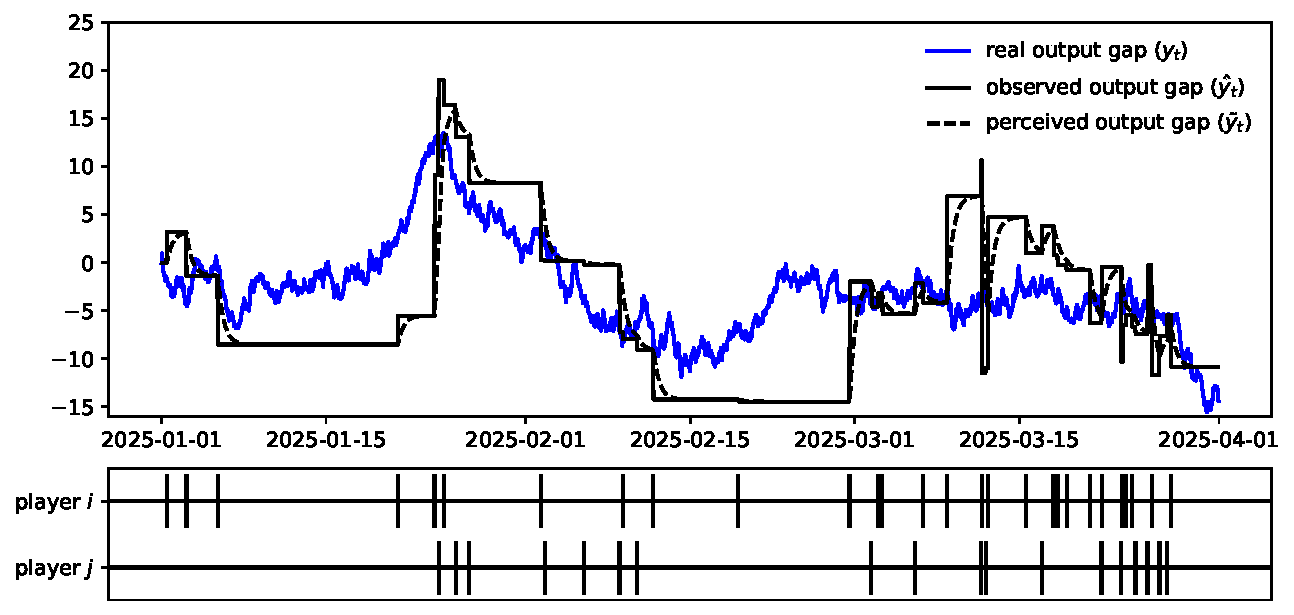
\includegraphics[scale=0.75]{synthetic_data.pdf}
	\caption{Synthetic Contest Data of Two Players from 2025-01-01 to 2025-04-01\\($\theta = 1.0$, $c_i = 1.2$, $c_j = 1.5$, $\sigma = 2.0$, $\lambda = 1.0$, $r = 15$)}
	\label{fig-synthetic_90}
\end{figure}

Figure~\ref{fig-synthetic_90} shows a realization of the virtual contest described above.
The blue line in Figure~\ref{fig-synthetic_90} represents the underline true output gap $y_t$, which can be interpreted as a \textit{private} leaderboard visible only to the contest designer, who has exclusive access to the full dataset.
Its drift is determined by the cumulative effort gap between the two players, while its volatility is governed by the contest’s innovation risk parameter $\sigma$. 
The solid black line depicts the corresponding \textit{public} leaderboard $\hat{y}_t$, which is updated whenever a submission is made by either player $i$ or $j$, as indicated by the short vertical ticks.
Intuitively, the more information is disclosed, the more closely the public leaderboard $\hat{y}_{t_k}$ approximates the true state $y_{t_k}$; the level of signal noise is controlled by the precision parameter $\lambda$.
The dashed black line shows the players’ perceived output gap $\tilde{y}_t$, as inferred from the public leaderboard and defined in equation~(\ref{eq-fintered-y-update}).
Submission times $\hat{t}^i_k$ and $\hat{t}^j_k$, marked by the short vertical ticks, are driven by each player’s effort level and are modelled as realizations of an inhomogeneous Poisson process.
There are 28 submissions from player $i$ and 18 submissions from player $j$. 

One might observe that, between two submissions $\hat{t}_{k}$ and $\hat{t}_{k+1}$, the estimate variance of the two players $S_t$ should increase over time rather than remain constant as we have assumed. 
However, under our modelling assumption where no submission implies low effort, a Bayesian player would infer that inactivity signals low intensity, thereby narrowing the estimation variance. 
For analytical tractability and to leverage the steady-state equilibrium formulation (\ref{eq-equilibrium-effort}), we abstract from modelling time-varying uncertainty.

Each parameter of $\Theta$ is assigned a truncated normal prior, with the choice of mean, variance, and support tailored to ensure numerical stability and to reflect the amount of prior information available.
Specifically, the prior distribution for each parameter $c_i$ and $c_j$ is specified as a truncated normal distribution bounded between 0.1 and 5, with a mean of 0.5 and variance of 5.
The prior for $\sigma$ follows a truncated normal distribution on the interval [0.5, 10], with mean 1 and variance 5.
Similarly, the prior for $\lambda$ supports on [1e-6, 10], also with mean 1 and variance 5.
The prior for $\mu_0$, by contrast, is more informative: it follows a truncated normal distribution over [-20, 20], centered at the observed initial value $\hat{y}_0$ with variance 1.
This reflects a stronger prior belief about the initial latent state and serves to anchor the model, thereby enhancing the stability and identifiability of the inference procedure.

\begin{table}[htbp]
\newcolumntype{Y}{>{\centering\arraybackslash}X}
\centering
\caption{Bayesian Estimates from Synthetic Data}\label{tbl-contest90}
\begin{tabularx}{\textwidth}{lYYYYY}
\toprule
\textbf{Parameters} & \textbf{$c_i$} & \textbf{$c_j$} & \textbf{$\sigma$} & \textbf{$\lambda$} & \textbf{$\mu_0$} \\
\addlinespace[0.25ex]
\cline{2-6}
\addlinespace[0.25ex]
(true val.)        & 1.2 & 1.5 & 2.0 & 1.0 & 0.0 \\
\midrule
 Posterior Mean    & 1.089 & 1.751 & 2.801 & 1.105 & 0.005 \\
 Posterior Stderr   & 0.258 & 0.476 & 0.503 & 0.299 & 0.990 \\
 RMSE                  & 0.281 & 0.538 & 0.945 & 0.317 & 0.990 \\
 95\% Interval        
		& [0.68, 1.68] 
		& [1.01, 2.85]
		& [1.95, 3.93]
		& [0.62, 1.78] 
		& [-1.92, 1.94] \\
\bottomrule
\addlinespace[0.5ex]
\end{tabularx}
\begin{minipage}{\textwidth}
{\footnotesize
\textit{Note:} (1) $\text{MSE}(\hat\theta) = \mathbb{E}(\hat{\theta}-\theta)^2 = [\mathbb{E}(\hat{\theta}) - \theta]^2 + Var(\hat{\theta})$ by the bias–variance decomposition. RMSE is then calculate by the squared root of MSE. 
(2) Players $i$ and $j$ submit 28 and 18 times respectively.
}
\end{minipage}
\end{table}

Table~\ref{tbl-contest90} presents the Bayesian inference results based on the synthetic data that we display in Figure~\ref{fig-synthetic_90}. 
Due to the limited data from the short contest duration, the posterior distribution of some parameters (such as $\sigma$ in this example) remains relatively far from the true value.
Nevertheless, given the limited sample size, the performance of Bayesian estimation is satisfactory. 
For most parameters (specifically $c_i$, $c_j$, $\lambda$ and $\mu_0$), the posterior means lie reasonably close to their true values.

We next examine whether Bayesian estimation improves with increasing data quantity.


\subsection{Asymptotic Properties}

With the synthetic contest data in place, it is important to ensure that our Bayesian framework is statistically coherent and implemented correctly. 
To this end, we numerically examine the asymptotic behaviour of the posterior distribution under two scenarios:
$i$) repeating the experiment multiple times under a fixed data-generating process, and $ii$) observing a single contest over an long time horizon.
As the amount of data increases, posterior consistency ensures that the Bayesian posterior concentrates around the true parameter values (\citealt{vaart1998asymptotic}, \citealt{ghosal2000convergence}, \citealt{pokern2013posterior}, \citealt{ramamoorthi2015posterior}).
While our analysis is simulation-based rather than theoretical, it provides evidence that the proposed likelihood formulation and inference procedure behave as expected in large-sample regimes.


\subsubsection{Replications.}

To begin, we investigate the asymptotic behavior of the posterior distribution when multiple independent realizations of the contest are observed. 
Multiple contests are independently simulated under identical parameters, with their data pooled to form a larger sample for Bayesian inference.
This setting corresponds to a replicated experimental design and allows us to assess whether Bayesian inference consistently recovers the true parameters as the number of observed contests increases.

The experimental results are presented in Table~\ref{tbl-pool-synthetic-data}. 
We replicate the contest simulation with 10 and 20 independent instances. 
Compared with Table~\ref{tbl-contest90}, we find that as the sample size increases, the RMSE of most parameters decreases, indicating that the posterior distributions converge more closely to the true parameter values.

\begin{table}[htbp]
\newcolumntype{Y}{>{\centering\arraybackslash}X}
\centering
\caption{Bayesian Estimates from Pooled Synthetic Data}\label{tbl-pool-synthetic-data}
\begin{tabularx}{\textwidth}{lYYYYY}
\toprule
\textbf{Parameters} & \textbf{$c_i$} & \textbf{$c_j$} & \textbf{$\sigma$} & \textbf{$\lambda$} & \textbf{$\mu_0$}\\
\addlinespace[0.25ex]
\cline{2-6}
\addlinespace[0.25ex]
(true val.)        & 1.2 & 1.5 & 2.0 & 1.0 & 0.0\\
\midrule
\addlinespace
\multicolumn{5}{l}{\textbf{Pool of 10 Contests}} \\
Posterior Mean  & 1.254 & 1.686 & 1.912 & 1.053 & -0.009\\
Posterior Stderr & 0.087 & 0.128 & 0.095 & 0.090 & 0.975\\
RMSE                & 0.102 & 0.225 & 0.130 & 0.104 & 0.975\\
\addlinespace
\multicolumn{5}{l}{\textbf{Pool of 20 Contests}} \\
Posterior Mean  & 1.204 & 1.639 & 1.981 & 0.988 & 0.008\\
Posterior Stderr & 0.060 & 0.089 & 0.068 & 0.060 & 1.003\\
RMSE                & 0.060 & 0.165 & 0.071 & 0.062 & 1.003\\
\bottomrule
\addlinespace[0.5ex]
\end{tabularx}
\begin{minipage}{\textwidth}
{\footnotesize
\textit{Note:} $\text{MSE}(\hat\theta) = \mathbb{E}(\hat{\theta}-\theta)^2 = [\mathbb{E}(\hat{\theta}) - \theta]^2 + Var(\hat{\theta})$ by the bias–variance decomposition. RMSE is then calculate by the squared root of MSE. 
}
\end{minipage}
\end{table}

%%%%%%%%%%%%%%%%%%%%%%%%%%%%%%%%%%%

\begin{table}[htbp]
\newcolumntype{Y}{>{\centering\arraybackslash}X}
\centering
\caption{Bayesian Estimates from Long Term Synthetic Data}\label{tbl-longterm-synthetic-data}
\begin{tabularx}{\textwidth}{lYYYYY}
\toprule
\textbf{Parameters} & \textbf{$c_i$} & \textbf{$c_j$} & \textbf{$\sigma$} & \textbf{$\lambda$} & \textbf{$\mu_0$}\\
\midrule
\multicolumn{5}{l}{\textbf{Contest of 6 Months}} \\
True Value           & 0.6     & 0.75   & 2.0     & 1.0     & 0.0\\
Posterior Mean    & 0.806 & 0.936 & 1.685 & 1.116 & 0.011\\
Posterior Stderr   & 0.112 & 0.142 & 0.148 & 0.171 & 0.986\\
RMSE                  & 0.234 & 0.234 & 0.348 & 0.207 & 0.986\\
\addlinespace
\multicolumn{5}{l}{\textbf{Contest of 12 Months}} \\
True Value           & 0.3     & 0.375 & 2.0     & 1.0     & 0.0\\
Posterior Mean    & 0.333 & 0.436 & 2.067 & 1.101 & 0.012\\
Posterior Stderr   & 0.027 & 0.046 & 0.097 & 0.138 & 0.994\\
RMSE                  & 0.043 & 0.076 & 0.118 & 0.171 & 0.994\\
\bottomrule
\addlinespace[0.5ex]
\end{tabularx}
\begin{minipage}{\textwidth}
{\footnotesize
\textit{Note:} (1) $\text{MSE}(\hat\theta) = \mathbb{E}(\hat{\theta}-\theta)^2 = [\mathbb{E}(\hat{\theta}) - \theta]^2 + Var(\hat{\theta})$ by the bias–variance decomposition. RMSE is then calculate by the squared root of MSE. 
(2) Players $i$ and $j$ submit 59 and 51 times in the 6-month contest, and 100 and 97 times in the 12-month contest, respectively.
}
\end{minipage}
\end{table}



\subsubsection{Long-Horizon Contest.}

We then turn to an alternative asymptotic regime in which a single contest instance is observed over a long time horizon. 
Rather than increasing the number of trajectories, we examine how the accumulation of submissions over a longer period improves inference accuracy. 

When generating long-horizon contest data, it is important to appropriately lower the effort costs $c_i$ and $c_j$ to ensure sustained effort from the contestants.
This is because effort levels are influenced by the remaining time until the deadline:
according to equation~(\ref{eq-equilibrium-effort}), the further away the deadline, the lower the equilibrium effort. 
Moreover, with volatility held constant, a long contest duration increases the likelihood that the true output gap undergoes a random walk to an unusually high level, potentially resulting in unexpected early success \citep{Ryvkin2022Fight}.
These factors may affect the quality of the generated data. 

Table~\ref{tbl-longterm-synthetic-data} presents simulations of contests lasting 6 and 12 months. 
In the 6-month contest, we set the unit effort costs to $c_i = 0.6$ and $c_j = 0.75$, resulting in 59 submissions from player $i$ and 51 from player $j$.
For the 12-month contest, the effort costs are reduced to $c_i = 0.3$ and $c_j = 0.375$, with players $i$ and $j$ submitting 100 and 97 times, respectively.
The posterior results show that longer contest durations and more frequent submissions lead to smaller RMSEs in the posterior distribution, indicating improved recovery of the true parameter values.




\section{Empirical Application}
\label{sec-kaggle-application}

In this section, we apply our model to multiple real-world Kaggle contests to evaluate the structural validity of the proposed theoretical contest model in Section~\ref{contest-theory} and the Bayesian estimation framework in Section~\ref{sect-bayes-framework}. 

We select a set of representative competitions from the Meta-Kaggle dataset and, for each contest, identify two focal participants $i$ and $j$ based on criteria such as submission frequency, activity duration, and final ranking.
Using the submission records and public leaderboard trajectories of the two players $i$ and $j$, we construct the observed data $\{t^i_k\}^{N_i}_{k=1}$, $\{t^j_k\}^{N_j}_{k=1}$ and $\{\hat{y}_{t_k}\}_{k=1}^{N_i+N_j}$.
Then, we perform Bayesian estimation for each of these contests under a unified prior specification.

To evaluate the structural validity of the model, we then conduct a cross-contest analysis using information not incorporated in the Bayesian inference—namely, the \textit{private} leaderboard scores $(y_t)$. 
These scores, which reflect the true performance of each submission but remain hidden from players during the contest, serve as an \textit{ex post} benchmark for evaluating model accuracy.
Specifically, we implement a cross-validation strategy by deriving alternative estimates of the contest-specific parameters $\lambda$ and $\sigma$ from the private leaderboard data $(y_t)$ and comparing them to the structural estimates from our Bayesian procedure, thereby assessing the empirical explanatory power of the theoretical model.
Figure~\ref{kaggledata-diagram} provides a schematic representation of the data-model structure and the cross-validation strategy used to assess model validity.

\begin{figure}[!ht]
	\centering
	\noindent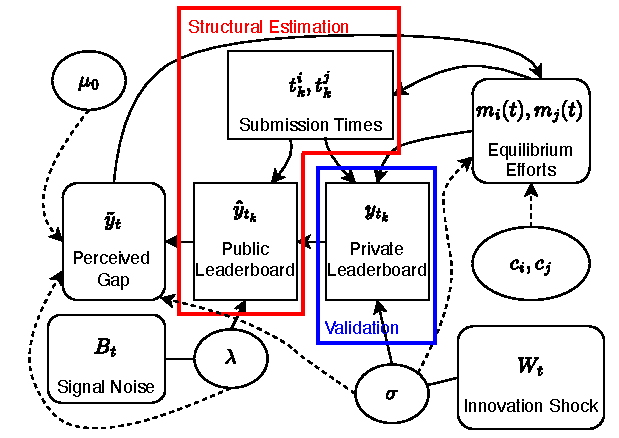
\includegraphics[scale=1.2]{kaggledata_diagram.pdf}
	\caption{Meta-Kaggle Dataset and the Model Structure}
	\label{kaggledata-diagram}
	\begin{minipage}{\textwidth}
{\footnotesize
\medskip
\textit{Note:} (1) Rectangles, rounded rectangles and ellipses represent observed data, latent states and parameters, respectively. 
(2) Solid lines depict relationships among variables of time series data and state variables; dashed arrows show the influence of contest parameters. 
}
\end{minipage}
\end{figure}


\subsection{Preparing Data for Structural Estimation}
\label{sec-data-clean}

To empirically implement the structural estimation framework developed in the previous sections using Kaggle data, the first step is to map the observed data onto the corresponding variables defined by the model.
This subsection details the procedures for selecting competitions, identifying key participants, and incorporating contest-specific information such as prize structures to make the data compatible with the model’s structural assumptions.

% Reward
As a first criterion for contest selection, we focus on the structure of monetary rewards.
Specifically, we restrict our attention to Kaggle competitions that award one, two, or three monetary prizes denominated in U.S. dollars.
Competitions offering a single prize naturally conform to the winner-take-all incentive structure. 
For those awarding two or three prizes, we standardize the reward structure to align with our theoretical model by focusing on the additional gain from winning, measured as the prize difference between the top two participants.

Unlike in our model, where the losing player receives nothing, non-winning players on Kaggle often gain symbolic recognition such as medals. 
These additional incentives introduce noise that complicates the identification of a clean winner-take-all setting.
By concentrating on the prize gap between the top two players, we mitigate such confounding factors and bring the empirical setting closer to the assumptions of our theoretical framework.

% Players
The second criterion requires that each contest allow for the identification of two top participants who engage in sustained and sufficiently intense competition throughout the contest period.
We begin by examining the final rankings on the private leaderboard and consider candidates from the top downward. 
To ensure rich strategic interaction along with adequate data that supports reliable estimation, we impose two conditions: (1) each participant must have submitted at least five times, and (2) their active periods must exhibit sufficient temporal overlap. 
The first condition ensures that a participant appears frequently enough on the public leaderboard to attract the attention of potential rivals, while the second guarantees that the two players competed over a shared and extended timeframe. 
These criteria help ensure that the observed data are informative and that the underlying dynamics are well-suited for reliable structural Bayesian inference.

While analytically convenient, restricting attention to two participants may limit representativeness, oversimplify the contest’s strategic environment, introduce hindsight bias via \textit{ex post} rankings, and overlook potential indirect influences from other contestants.

However, this approach remains feasible in the Kaggle context, where participants typically have access to ample information about their rivals. 
Team compositions are publicly available, and individual profiles include detailed historical records such as past rankings, medal counts, and shared notebooks that allow players to quickly gauge the technical abilities of their competitors. 
Additionally, forum discussions and public notebooks foster a semi-transparent environment in which ideas and strategies are informally exchanged. 
These features collectively enable top teams to identify potential competitors and adjust their strategies accordingly. 

% Leaderboard Display
The third criterion for contest selection concerns the format in which leaderboard scores are presented.
Since Kaggle competitions are based on diverse real-world tasks, the scoring metrics vary accordingly.
Some are based on raw scores (positive real numbers), while others are based on accuracy measures (expressed as percentages or decimals between 0 and 1).
Ignoring these differences would lead to inconsistencies in units across contests, complicating any meaningful cross-contest comparison of parameter estimates.

After careful evaluation, we find that contests reporting accuracy-based scores (i.e., values between 0 and 1 on the leaderboard) tend to yield a higher success rate in identifying two focal players.
Therefore, all contests used in this study are restricted to those where the leaderboard displays accuracy scores.
To ensure consistency with the theoretical definition of the performance gap variable $y_t$ and $\hat{y}_t$, we further transform the raw leaderboard accuracy values using the logit (log-odds) function: 
\begin{equation}\label{eq-leaderboard-transform}
y_t = a \cdot \log\left(\frac{p_t}{1-p_t}\right), \quad p_t\in[0.5, 1)
\end{equation}
where $p_t$ is the leaderboard score, and $a$ is a tune parameter for the normality of $y_t$.\footnote{
For different contest data, parameter $a$ is different. 
 The goal is to make the transformed data more consistent with the normality assumption in (\ref{eq-state-dynamics}).
In practise, we just pick $a = 1$. 
}
The logit function is S-shaped, with the key property that as the accuracy $p_t$ approaches 1, each marginal improvement in $p_t$ results in a disproportionately large increase in the transformed value $y_t$. 
This feature aligns with the intuition that it becomes increasingly difficult to improve performance near the upper bound, making such gains more informative in competitive settings.


\subsection{Structural Validation}


We select 75 contests from the Meta-Kaggle database, encompassing all eligible competitions concluded before April 15, 2025.\footnote{
The Meta-Kaggle database is updated daily, with new competition data added after the contests conclude.
}
For each selected contest, we successfully identify two top participants who meet our criteria.
Appendix~\ref{appendix-statistics} reports the Bayesian estimation results for each contest individually.

We next perform a cross-validation of the contest-specific parameters using data from the private leaderboard.

\subsubsection{Cross-Validation of Signal's Precision $\lambda$.}

The signal precision parameter $\lambda$ is a prototypical contest-specific variable, influenced by factors such as the proportion of public leaderboard data relative to the full dataset, the sampling mechanism, and the distributional characteristics of the data.
We assume that each participant has a rough understanding of the signal precision, and thus it plays a role in shaping their strategic behavior.
The parameter $\lambda$ can be inferred in two ways: structurally, through Bayesian estimation based on submissions $\{t^i_k\}_{k=1}^{N_i}$, $\{t^j_k\}_{k=1}^{N_j}$ and public leaderboard trajectories $\{\hat{y}_{k}\}_{k=1}^{N_i+N_j}$; or non-structurally, by directly comparing the discrepancies between the public and private leaderboards.

Let $c = {1, 2, ... }$ index the contest.
Based on the data-generating process described in equation~(\ref{eq-leaderboard-gap}), we can derive a straightforward maximum likelihood estimator (MLE) for the true value of $\lambda_c$.
Given that the discrepancy between the public and private leaderboard scores satisfies $\hat{y}_k^c - y_k^c \sim \mathcal{N}(0, 1/(\lambda_c\Delta))$, $\forall k = 1, 2, ..., N^c$, we have 
\begin{equation*}
\lambda^{\text{MLE}}_c = \frac{N^c}{\Delta\sum^{N^c}_{k=1}(y_k^c - \hat{y}_k^c)^2}, \quad N^c = N^c_i + N^c_j
\end{equation*}
Here, $N^c_i$ and $N^c_j$ denotes for the number of submissions of player $i$ and $j$ in contest $c$. 

It is important to emphasize that the normality assumption in this setting is induced by the transformation defined in equation~(\ref{eq-leaderboard-transform}). 
However, the current transformation form is adopted for simplicity, and does not guarantee strict normality—especially under extreme contest data—which may reduce the validity of our MLE.\footnote{So far, only half of the contest data can pass the Shapiro-Wilk test. }
Future work should explore more reliable transformation methods to better approximate the assumed distribution.

Next, we regress the non-structural benchmark $\lambda^{\text{MLE}}$ on the Bayesian structural estimates $\hat\lambda$ to examine whether a positive relationship holds between the two.
The following table reports the results from this regression analysis: 

%%%%%%%%%% Figure & Table %%%%%%%%%%%
\noindent
\begin{minipage}[t]{0.43\textwidth}
	\vspace*{\fill}
	\centering
	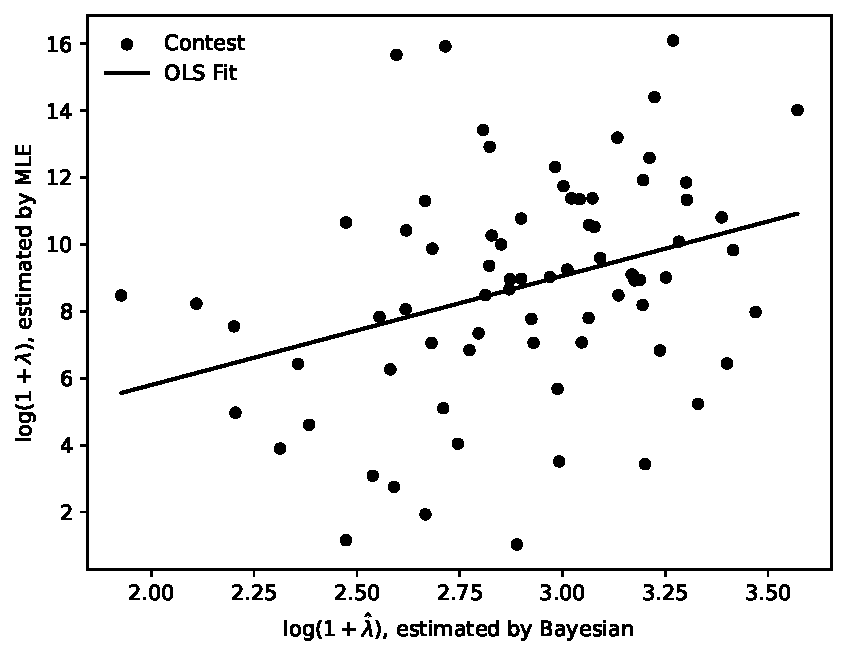
\includegraphics[width=\linewidth]{validate_lamb.pdf}
	\vspace*{\fill}
\end{minipage}
\hfill
\begin{minipage}[t]{0.53\textwidth}
	\vspace*{\fill}
	\centering
	\newcolumntype{Y}{>{\centering\arraybackslash}X}
	\begin{tabularx}{\textwidth}{llYY}
		\toprule
		& coef. & stderr & 95\% CI \\
		\midrule
		const.
		& -0.733 & 3.182 & [-7.07, 5.61] \\
		$\log(1 + \hat{\lambda})$ 
		& 3.264\textbf{**} & 1.088 & [1.10, 5.43] \\
		\midrule
		Obs. & \multicolumn{3}{c}{75} \\
		R$^2$ & \multicolumn{3}{c}{0.110} \\
		Adj. R$^2$ & \multicolumn{3}{c}{0.098} \\
		\bottomrule
		\addlinespace[0.5ex]
	\end{tabularx}
	\begin{minipage}{\textwidth}
{\footnotesize
\textit{Note:} (1) Significance levels: \textbf{***} $p < 0.001$, \textbf{**} $p < 0.01$, \textbf{*} $p < 0.05$. 
(2) Normality diagnostics: Omnibus = 0.378, Jarque-Bera = 0.071, Skewness = -0.042, Kurtosis = 3.126. 
(3) Other diagnostic statistics: Condition Number = 28.2, Durbin-Watson = 2.244.
}
	\end{minipage}
	\vspace*{\fill}
\end{minipage}
%%%%%%%%%%%% Captions %%%%%%%%%%%%
\noindent
\begin{minipage}[t]{\textwidth}
	\centering
	\captionof{figure}{$\lambda^{\text{MLE}}$ vs. Bayesian Estimate $\hat\lambda$}
	\label{fig-validate-lambda}
\end{minipage}
%\hfill
%\begin{minipage}[t]{0.53\textwidth}
%	\centering
%	\captionof{table}{Regression of $\lambda^{\text{MLE}}$ on Bayesian Estimate $\hat\lambda$}
%\end{minipage}
\medskip

The left panel of Figure~\ref{fig-validate-lambda} reveals a clear positive relationship between the log-transformed estimates of $\hat\lambda$ and $\lambda^{\text{MLE}}$.
In the accompanying regression table, we observe that the intercept is statistically insignificant, while the slope coefficient is estimated at 3.288 and is statistically significant at the 1\% level. 
The regression residuals exhibit no significant deviation from normality, as indicated by the low Jarque-Bera statistic (0.071), near-zero skewness (-0.042), and kurtosis close to 3 (3.126). 
The condition number (28.2) suggests no severe multicollinearity, while the Durbin-Watson statistic (2.244) indicates no significant autocorrelation in the residuals. 
These diagnostics support the validity of the OLS assumptions.

It is worth noting, however, that the $R^2$ of the regression is relatively low, around 0.1, suggesting that the scatter points are not tightly clustered around the fitted line but instead show substantial dispersion.
This pattern likely reflects the limited sample size as well as the simplifying assumptions introduced during data processing and structural estimation.




\subsubsection{Cross-Validation of Innovation Risk $\sigma$.}

Another key contest-specific parameter is $\sigma$, which captures the degree of uncertainty in the data analysis and algorithm innovation process. 
A larger $\sigma$ implies that chance plays a greater role compared to effort, and that the outcomes of innovation are more unpredictable. 
From the perspective of contest participants, the overall uncertainty associated with the real-world task is typically anticipated to some extent, and this perception can influence their strategic behaviour.
We estimate $\hat{\sigma}_c$ structurally via Bayesian inference for each contest $c$, using the public submission records of the two participants, denoted jointly as $\{t_k^c\}_{k=1}^{N^c_i + N^c_j}$, together with the corresponding public leaderboard trajectories $\{\hat{y}_{k}\}_{k=1}^{N^c_i + N^c_j}$. 
In addition, a more direct and model-free estimate of $\sigma$ can be obtained by measuring the volatility of the private leaderboard scores $\{y_k\}_{k=1}^{N^c_i+N^c_j}$.

Since the private leaderboard dynamics (\ref{eq-state-dynamics}) are modelled as a diffusion process drifted by effort gap, it follows that $y^c_{k+1} - y^c_{k} \sim \mathcal{N}\left(\mu^c_k, \sigma^2(t^c_{k+1}-t^c_k)\right)$ where $\mu^c_k = \int^{t^c_{k+1}}_{t^c_k}m^c_i(s) - m^c_j(s)ds$. 
Given this, we derive the maximum likelihood estimator (MLE) of the contest-specific parameter $\sigma$ (see Appendix~\ref{appexidx-normal-MLE} for the derivation): 
\begin{equation*}
\sigma^{\text{MLE}}_c = \left(\frac{1}{N^c_i+N^c_j}\sum_k\frac{\left[y^c_{k+1}-y^c_{k}-\hat\mu^c_k\right]^2}{t^c_{k+1}-t^c_k}\right)^{1/2}
\end{equation*}
where $\hat\mu^c_k$ is retrieved from the Bayesian posterior estimates of the effort trajectories for the two players.

As in the analysis above for $\lambda$, we regress $\sigma^{\text{MLE}}$ on the structural estimate $\hat{\sigma}$ to examine whether a significant positive relationship exists between the two. 
The regression results are presented in the table below:

%%%%%%%%%% Figure & Table %%%%%%%%%%%
\noindent
\begin{minipage}[t]{0.43\textwidth}
	\vspace*{\fill}
	\centering
	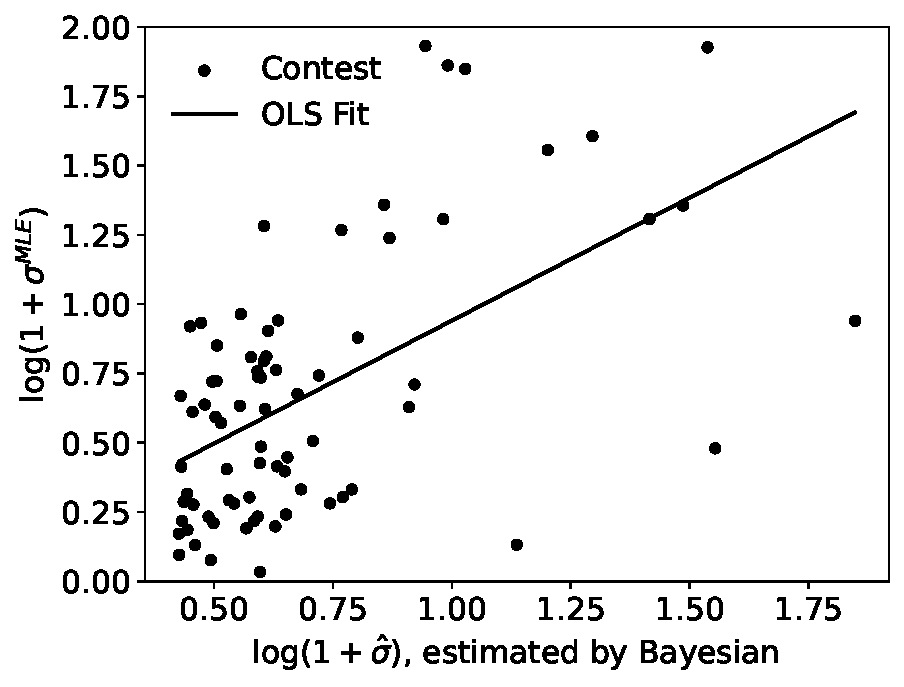
\includegraphics[width=\linewidth]{validate_sigma.pdf}
	\vspace*{\fill}
\end{minipage}
\hfill
\begin{minipage}[t]{0.53\textwidth}
	\vspace*{\fill}
	\centering
	\newcolumntype{Y}{>{\centering\arraybackslash}X}
	\begin{tabularx}{\textwidth}{llYY}
		\toprule
		& coef. & stderr & 95\% CI \\
		\midrule
		const.
		& 0.054 & 0.116 & [-0.18, 0.29] \\
		$\log(1 + \hat{\lambda})$ 
		& 0.887\textbf{***} & 0.152 & [0.58, 1.19] \\
		\midrule
		Obs. & \multicolumn{3}{c}{75} \\
		R$^2$ & \multicolumn{3}{c}{0.317} \\
		Adj. R$^2$ & \multicolumn{3}{c}{0.308} \\
		\bottomrule
		\addlinespace[0.5ex]
	\end{tabularx}
	\begin{minipage}{\textwidth}
{\footnotesize
\textit{Note:} (1) Significance levels: \textbf{***} $p < 0.001$, \textbf{**} $p < 0.01$, \textbf{*} $p < 0.05$. 
(2) Normality diagnostics: Omnibus = 1.280, Jarque-Bera = 0.774, Skewness = 0.225, Kurtosis = 3.214.
(3) Other diagnostic statistics: Condition Number = 5.08, Durbin-Watson = 1.618.
}
	\end{minipage}
	\vspace*{\fill}
\end{minipage}
%%%%%%%%%%%% Captions %%%%%%%%%%%%
\noindent
\begin{minipage}[t]{\textwidth}
	\centering
	\captionof{figure}{$\sigma^{\text{MLE}}$ vs. Bayesian Estimate $\hat\sigma$}
	\label{fig-validation-sigma}
\end{minipage}
\medskip

The left panel of Figure~\ref{fig-validation-sigma} reveals a clear positive relationship between the log-transformed estimates of $\hat{\sigma}$ and $\sigma^{\text{MLE}}$. 
In the accompanying regression results, the intercept is small and statistically insignificant, while the slope coefficient on $\log(1 + \hat{\sigma})$ is estimated at 0.887 and is highly significant at the 0.1\% level. 
This indicates a strong positive association between the structural and non-structural estimates of the uncertainty parameter $\sigma$.
The residual diagnostics indicate no major violations of the classical OLS assumptions. 
Normality appears reasonable, as evidenced by the Omnibus statistic (1.280), Jarque-Bera test (0.774), moderate skewness (0.225), and a kurtosis value close to 3 (3.214). 
The condition number (5.08) rules out serious multicollinearity, and the Durbin-Watson statistic (1.618) suggests no significant autocorrelation in the residuals.
Moreover, compared to the earlier analysis of $\lambda$, the model fit here is notably stronger: the regression yields an $R^2$ above 0.3, indicating a moderately good fit. 


\section{Robustness}

...

\subsection{Selection of Two Players}\label{sect-robust-2players}

One plausible conjecture is that each contestant perceives themselves as competing against an imagined strongest opponent. 
This perceived benchmark is likely shaped by the public leaderboard performances of several genuinely strong teams, while also being influenced by the top-ranked submission, which often exhibits substantial overfitting to the public leaderboard.

\subsubsection{1-3.}

...

%%%%%%%%%% Figure & Table %%%%%%%%%%%
\noindent
\begin{minipage}[t]{0.43\textwidth}
	\vspace*{\fill}
	\centering
	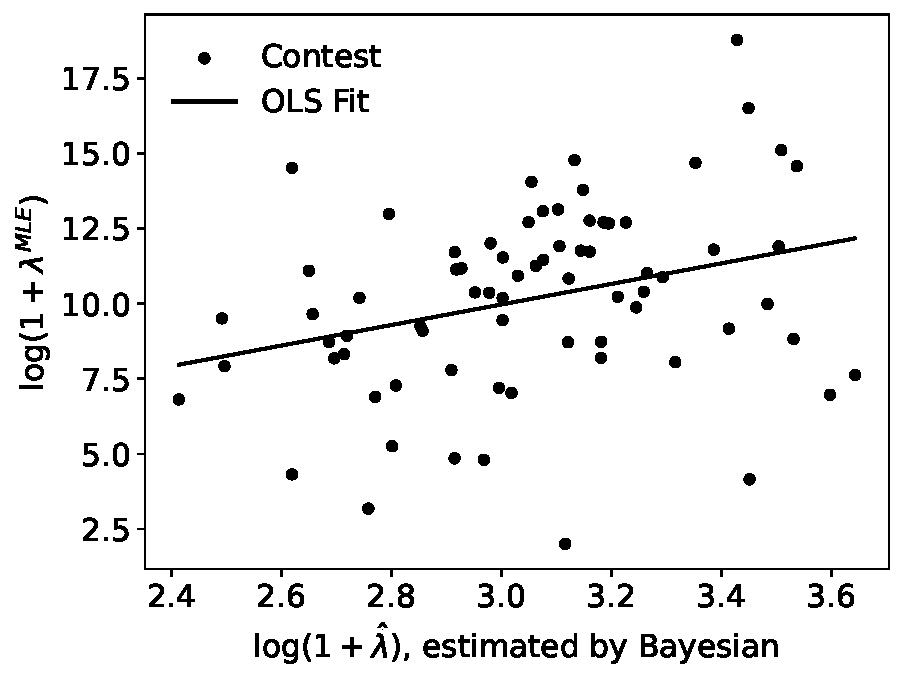
\includegraphics[width=\linewidth]{validate_lamb_robust13.pdf}
	\vspace*{\fill}
\end{minipage}
\hfill
\begin{minipage}[t]{0.53\textwidth}
	\vspace*{\fill}
	\centering
	\newcolumntype{Y}{>{\centering\arraybackslash}X}
	\begin{tabularx}{\textwidth}{llYY}
		\toprule
		& coef. & stderr & 95\% CI \\
		\midrule
		const.
		& 2.259 & 4.567 & [-6.85, 11.37] \\
		$\log(1 + \hat{\lambda})$ 
		& 2.551\textbf{***} & 1.490 & [xxx, xxx] \\
		\midrule
		Obs. & \multicolumn{3}{c}{75} \\
		R$^2$ & \multicolumn{3}{c}{xxx} \\
		Adj. R$^2$ & \multicolumn{3}{c}{xxx} \\
		\bottomrule
		\addlinespace[0.5ex]
	\end{tabularx}
	\begin{minipage}{\textwidth}
{\footnotesize
\textit{Note:} (1) Significance levels: \textbf{***} $p < 0.001$, \textbf{**} $p < 0.01$, \textbf{*} $p < 0.05$. 
(2) Normality diagnostics: Omnibus = xxx, Jarque-Bera = xxx, Skewness = xxx, Kurtosis = xxx.
(3) Other diagnostic statistics: Condition Number = xxx, Durbin-Watson = xxx.
}
	\end{minipage}
	\vspace*{\fill}
\end{minipage}
%%%%%%%%%%%% Captions %%%%%%%%%%%%
\noindent
\begin{minipage}[t]{\textwidth}
	\centering
	\captionof{figure}{$\lambda^{\text{MLE}}$ vs. Bayesian Estimate $\hat\lambda$}
	\label{fig-validation-lambda-robust13}
\end{minipage}
\medskip

...

%%%%%%%%%% Figure & Table %%%%%%%%%%%
\noindent
\begin{minipage}[t]{0.43\textwidth}
	\vspace*{\fill}
	\centering
	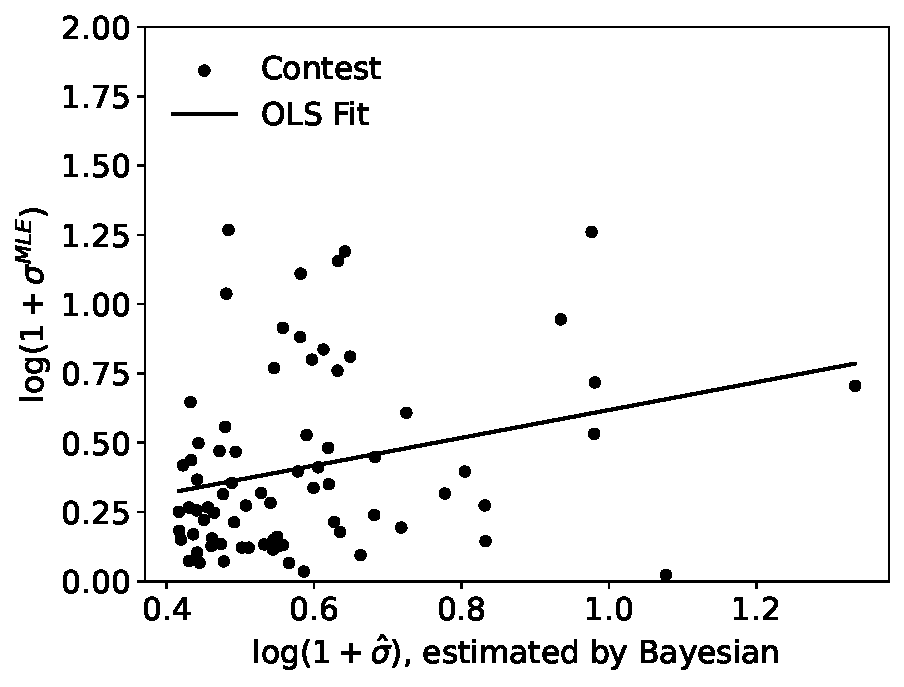
\includegraphics[width=\linewidth]{validate_sigma_robust13.pdf}
	\vspace*{\fill}
\end{minipage}
\hfill
\begin{minipage}[t]{0.53\textwidth}
	\vspace*{\fill}
	\centering
	\newcolumntype{Y}{>{\centering\arraybackslash}X}
	\begin{tabularx}{\textwidth}{llYY}
		\toprule
		& coef. & stderr & 95\% CI \\
		\midrule
		const.
		& xxx & xxx & [xxx, xxx] \\
		$\log(1 + \hat{\lambda})$ 
		& xxx\textbf{***} & xxx & [xxx, xxx] \\
		\midrule
		Obs. & \multicolumn{3}{c}{75} \\
		R$^2$ & \multicolumn{3}{c}{xxx} \\
		Adj. R$^2$ & \multicolumn{3}{c}{xxx} \\
		\bottomrule
		\addlinespace[0.5ex]
	\end{tabularx}
	\begin{minipage}{\textwidth}
{\footnotesize
\textit{Note:} (1) Significance levels: \textbf{***} $p < 0.001$, \textbf{**} $p < 0.01$, \textbf{*} $p < 0.05$. 
(2) Normality diagnostics: Omnibus = xxx, Jarque-Bera = xxx, Skewness = xxx, Kurtosis = xxx.
(3) Other diagnostic statistics: Condition Number = xxx, Durbin-Watson = xxx.
}
	\end{minipage}
	\vspace*{\fill}
\end{minipage}
%%%%%%%%%%%% Captions %%%%%%%%%%%%
\noindent
\begin{minipage}[t]{\textwidth}
	\centering
	\captionof{figure}{$\sigma^{\text{MLE}}$ vs. Bayesian Estimate $\hat\sigma$}
	\label{fig-validation-lambda-robust13}
\end{minipage}
\medskip

...

\subsubsection{2-3}

...

%%%%%%%%%% Figure & Table %%%%%%%%%%%
\noindent
\begin{minipage}[t]{0.43\textwidth}
	\vspace*{\fill}
	\centering
	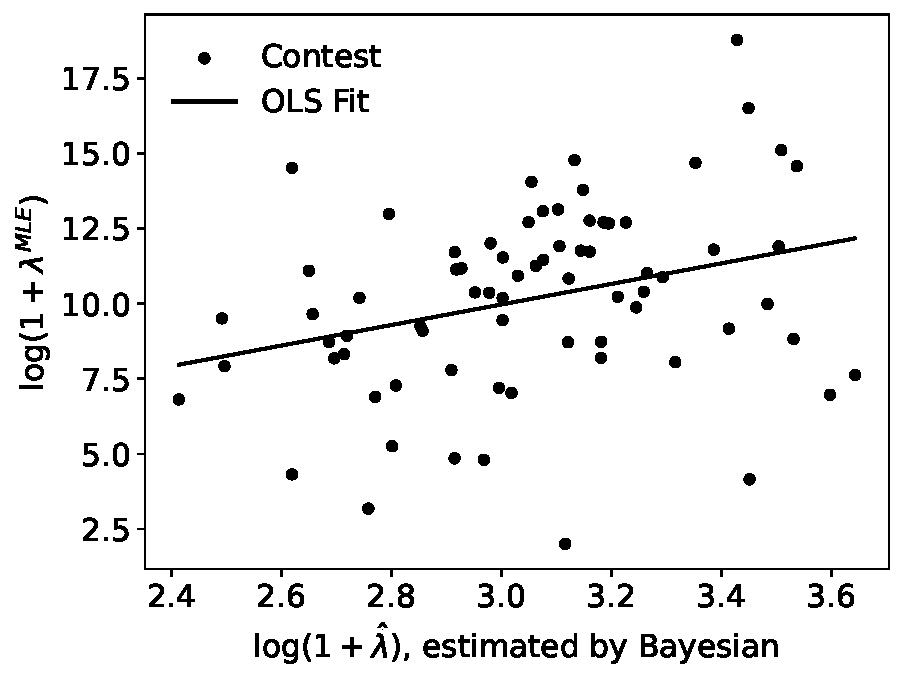
\includegraphics[width=\linewidth]{validate_lamb_robust23.pdf}
	\vspace*{\fill}
\end{minipage}
\hfill
\begin{minipage}[t]{0.53\textwidth}
	\vspace*{\fill}
	\centering
	\newcolumntype{Y}{>{\centering\arraybackslash}X}
	\begin{tabularx}{\textwidth}{llYY}
		\toprule
		& coef. & stderr & 95\% CI \\
		\midrule
		const.
		& 0.290 & 3.819 & [-7.91, 7.32] \\
		$\log(1 + \hat{\lambda})$ 
		& 3.421\textbf{***} & 1.244 & [0.94, 5.90] \\
		\midrule
		Obs. & \multicolumn{3}{c}{73} \\
		R$^2$ & \multicolumn{3}{c}{0.096} \\
		Adj. R$^2$ & \multicolumn{3}{c}{0.084} \\
		\bottomrule
		\addlinespace[0.5ex]
	\end{tabularx}
	\begin{minipage}{\textwidth}
{\footnotesize
\textit{Note:} (1) Significance levels: \textbf{***} $p < 0.001$, \textbf{**} $p < 0.01$, \textbf{*} $p < 0.05$. 
(2) Normality diagnostics: Omnibus = 3.192, Jarque-Bera = 2.424, Skewness = -0.411, Kurtosis = 3.350.
(3) Other diagnostic statistics: Condition Number = 36.9, Durbin-Watson = 2.236.
}
	\end{minipage}
	\vspace*{\fill}
\end{minipage}
%%%%%%%%%%%% Captions %%%%%%%%%%%%
\noindent
\begin{minipage}[t]{\textwidth}
	\centering
	\captionof{figure}{$\lambda^{\text{MLE}}$ vs. Bayesian Estimate $\hat\lambda$}
	\label{fig-validation-lambda-robust23}
\end{minipage}
\medskip

...

%%%%%%%%%% Figure & Table %%%%%%%%%%%
\noindent
\begin{minipage}[t]{0.43\textwidth}
	\vspace*{\fill}
	\centering
	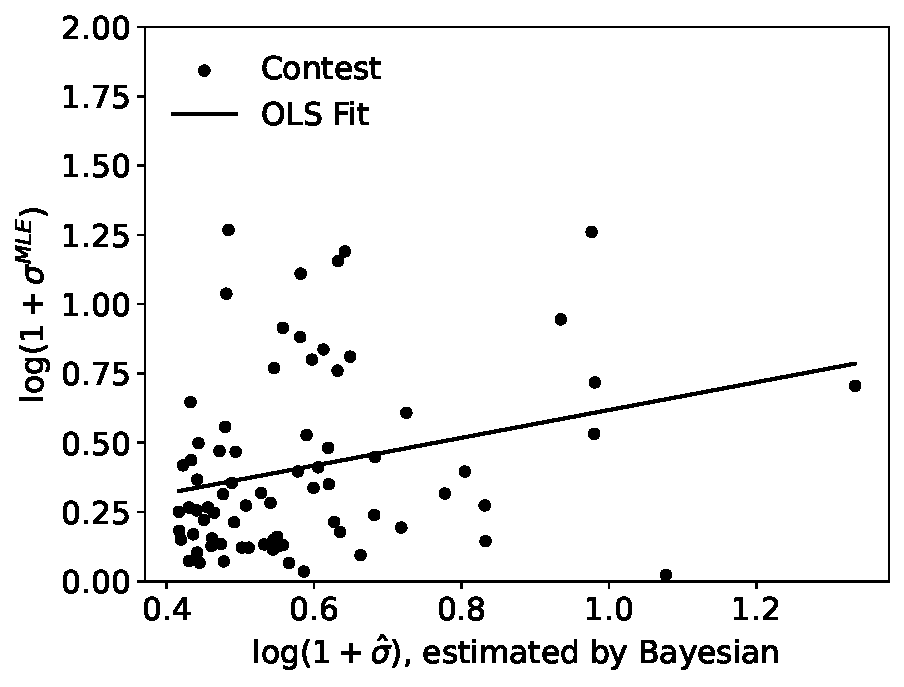
\includegraphics[width=\linewidth]{validate_sigma_robust23.pdf}
	\vspace*{\fill}
\end{minipage}
\hfill
\begin{minipage}[t]{0.53\textwidth}
	\vspace*{\fill}
	\centering
	\newcolumntype{Y}{>{\centering\arraybackslash}X}
	\begin{tabularx}{\textwidth}{llYY}
		\toprule
		& coef. & stderr & 95\% CI \\
		\midrule
		const.
		& 0.117 & 0.130 & [-0.14, 0.38] \\
		$\log(1 + \hat{\lambda})$ 
		& 0.501\textbf{***} & 0.212 & [0.08, 0.92] \\
		\midrule
		Obs. & \multicolumn{3}{c}{75} \\
		R$^2$ & \multicolumn{3}{c}{0.071} \\
		Adj. R$^2$ & \multicolumn{3}{c}{0.059} \\
		\bottomrule
		\addlinespace[0.5ex]
	\end{tabularx}
	\begin{minipage}{\textwidth}
{\footnotesize
\textit{Note:} (1) Significance levels: \textbf{***} $p < 0.001$, \textbf{**} $p < 0.01$, \textbf{*} $p < 0.05$. 
(2) Normality diagnostics: Omnibus = 12.72, Jarque-Bera = 13.66, Skewness = 1.02, Kurtosis = 3.50.
(3) Other diagnostic statistics: Condition Number = 7.84, Durbin-Watson = 1.87.
}
	\end{minipage}
	\vspace*{\fill}
\end{minipage}
%%%%%%%%%%%% Captions %%%%%%%%%%%%
\noindent
\begin{minipage}[t]{\textwidth}
	\centering
	\captionof{figure}{$\sigma^{\text{MLE}}$ vs. Bayesian Estimate $\hat\sigma$}
	\label{fig-validation-lambda-robust23}
\end{minipage}
\medskip



\subsection{}\label{sect-robust-normality}

...




\section{Conclusion}

% what we did
This paper develops a dynamic game-theoretic model and a Bayesian structural estimation framework tailored to online crowdsourcing contests.
% more...
The model captures how participants adjust their efforts in response to evolving public feedback and strategic competition, enabling the recovery of key latent components including perceived competition state, effort dynamics, individual abilities, innovation uncertainty, and signal precision based on in-contest data.
% what we find
Empirically, we apply the framework to 75 Kaggle contests and validate the structural estimates through a cross-validation strategy that uses outcome data excluded from the estimation stage but governed by the same underlying process.
We find strong and significant correlations between the estimated parameters and independent benchmarks, supporting the empirical validity of the model.


% limitations
Nonetheless, several limitations deserve mention.
% 1. DGP
First, the estimation relies on assumptions about the data-generating process (DGP) that may not fully reflect real-world complexities.
For example:
% - prize
(1) many contests use multi-tier or team-based prizes rather than the winner-take-all format assumed here;
% - players
(2) we focus on two-player settings, while actual contests involve broader participation;
% - leaderboard display
(3) leaderboard scores vary in format, complicating their integration into a unified signal structure.
% 2. Kalman-filter
Second, the estimation method simplifies belief updating by assuming the inference variance quickly converges and remains constant.
A more realistic approach would allow inference precision to evolve over time, e.g., via hybrid Kalman filtering, but such extensions would increase analytical complexity.
% Future
These limitations point to valuable directions for future work, including incorporating richer prize structures, multi-agent dynamics, and more flexible learning mechanisms to enhance realism and applicability.




% Appendix here
% Options are (1) APPENDIX (with or without general title) or
%             (2) APPENDICES (if it has more than one unrelated sections)
% Outcomment the appropriate case if necessary
%
% \begin{APPENDIX}{<Title of the Appendix>}
% \end{APPENDIX}
%
%   or
%
% \begin{APPENDICES}
% \section{<Title of Section A>}
% \section{<Title of Section B>}
% etc
% \end{APPENDICES}


\newpage
\begin{APPENDICES}


\section{Proofs}

\proof{Proof of Lemma~\ref{lmm-params-identifiability}}
Suppose $\Theta = (c_i, c_j, \mu_0, \sigma, \lambda)$ and $\Theta' = (c'_i, c'_j, \mu_0', \sigma', \lambda')$. 
To show that the model parameters are jointly identifiable, it suffices to show that 
\begin{equation*}
\mathcal{L}(\{\hat{t}^i_k\}_{k=1}^{N_i}, \{\hat{t}^j_k\}_{k=1}^{N_j}, \{\hat{y}_k\}_{k=1}^{N} | \Theta) = \mathcal{L}(\{\hat{t}^i_k\}_{k=1}^{N_i}, \{\hat{t}^j_k\}_{k=1}^{N_j}, \{\hat{y}_k\}_{k=1}^{N} | \Theta')
\Rightarrow
\Theta = \Theta'
\end{equation*}
where $N = N_i+N_j$ and $\mathcal{L}$ is the likelihood of observations given by (\ref{eq-ihpp-prob}) and (\ref{eq-obs_gap-prob}). 
First of all, let $\tau$ and $\tau'$ denotes for the intensity under $\Theta$ and $\Theta'$, $\mu_k$ and $\mu_k'$ the two mean term of $\hat{y}_{t_k}$,
we can write down the difference of the two log likelihoods:
\begin{equation*}
\begin{aligned}
0 &= \int_{s\in\mathcal{T}}\tau_i(s)ds \sum^{N_i}_{k=1}\log\tau_i(\hat{t}^i_k) - \int_{s\in\mathcal{T}}\tau'_i(s)ds \sum^{N_i}_{k=1}\log\tau'_i(\hat{t}^i_k) \\
&+ \int_{s\in\mathcal{T}}\tau_j(s)ds \sum^{N_j}_{k=1}\log\tau_j(\hat{t}^j_k) - \int_{s\in\mathcal{T}}\tau'_j(s)ds \sum^{N_j}_{k=1}\log\tau'_j(\hat{t}^j_k) \\ 
&+ \frac{1}{2}\log\left(\frac{\det\left(\Sigma_y+I_N/(\Delta \lambda)\right)}{\det\left(\Sigma_y+I_N/(\Delta\lambda')\right)}\right) \\
&+ \frac{1}{2}\Bigg\{\left(\left\{\hat{y}_k - \mu_k\right\}^{N}_{k=1}\right)^T\left(\Sigma_y+\frac{I_N}{\Delta\lambda}\right)\left\{\hat{y}_k - \mu_k\right\}^{N}_{k=1}
- \left(\left\{\hat{y}_k - \mu'_k\right\}^{N}_{k=1}\right)^T\left(\Sigma_y+\frac{I_N}{\Delta\lambda'}\right)\left\{\hat{y}_k - \mu'_k\right\}^{N}_{k=1}\Bigg\}
\end{aligned}
\end{equation*}
The first row of above is a function of $\{\hat{t}^i_k\}_{k=1}^{N_i}$, second row is a function of $\{\hat{t}^j_k\}_{k=1}^{N_j}$, second row is a constant while the forth row is a function of all dataset. 

Now, suppose we have $\{\hat{t}^i_k\}_{k=1}^{N_i}$ and $\{\hat{t}^j_k\}_{k=1}^{N_j}$ such that the summation of first three rows are exactly zero, then, the last two rows form a quadratic function of $\{\hat{y}_k\}_{k=1}^{N}$. 
The quadratic function is always zero only if all its coefficients are zero. 
Hence, we conclude that $\mu_k = \mu'_k$ and $\lambda = \lambda'$ and $\sigma = \sigma'$. 

Next, we consider the first row. If the sample size of $\{\hat{t}^i_k\}_{k=1}^{N_i}$ is empty, i.e., $N_i=0$, we conclude that the cumulative intensity of player $i$ is same, i.e., $\int_{s\in\mathcal{T}}\tau_i(s)ds = \int_{s\in\mathcal{T}}\tau'_i(s)ds$. 
By increasing $N_i$ by one, two, ..., we conclude that the evaluations of $\tau_i$ and $\tau'_i$ at all points are the same. 
Since the realization of $\hat{t}^i_k$ is random, we conclude that $\tau_i = \tau'_i$. 
Similarly, we have $\tau_j = \tau'_j$. 
It suffices to show that the mapping from $\Theta$ to function $\tau$ is an injection. 
Since $\sigma = \sigma'$ and $\lambda = \lambda'$, by the form of (\ref{eq-equilibrium-effort}), it is easy to show that if $\theta/c_i\not=\theta/c'_i$ or $\theta/c_j\not=\theta/c'_j$, we must have $m_i\not=m'_i$, implying that $\tau_i\not=\tau_j$. 
Furthermore, by the form of (\ref{eq-fintered-y-update}), we conclude that $\tau_i\not=\tau_j$ if $\mu_0\not=\mu'_0$. 
\Halmos
\endproof






\section{Auxiliary Results}

\subsection{Solve $S_t$ in Equation (\ref{filtered-S})}\label{app-S-equ}

If $S$ is in steady state $dS/dt = 0$ $\Leftrightarrow$ $S = \bar{S} \equiv \sigma/\sqrt{\lambda}$. 
If $S$ is not in steady state, i.e. $S\not=\bar{S}$, we first isolate the two variables and get 
\begin{equation*}
	\frac{dS}{\sigma-\lambda S^2} = dt
\end{equation*}
Then, we take the integral on both sides
\begin{equation*}
    t = \int \frac{dS}{\sigma-\lambda S^2} = \frac{1}{\sigma\sqrt{\lambda}} \int \frac{dS\sqrt{\lambda}/\sigma}{1 - (S\sqrt{\lambda}/\sigma)^2} \equiv \frac{1}{\sigma\sqrt{\lambda}}\int \frac{du}{1-u^2} 
\end{equation*}
where $u = S\sqrt{\lambda}/\sigma = S/\bar{S}$. Hence, 
\begin{equation*}
    \sigma\sqrt{\lambda}\cdot t = \begin{cases}
        \tanh^{-1}(u)-K_1, & \text{if } |u|<1\\
        \coth^{-1}(u)-K_2, & \text{if } |u|>1
    \end{cases} = \begin{cases}
        \tanh^{-1}(S/\bar{S})-K_1, & \text{if } S<\bar{S}\\
        \coth^{-1}(S/\bar{S})-K_2, & \text{if } S>\bar{S} 
\end{cases}
\end{equation*}
Thus, we conclude the non-steady state case that 
\begin{equation*}
	S = \begin{cases}
		\bar{S}\cdot\tanh(\sigma\sqrt{\lambda}\cdot t + K_1), & \text{if } S<\bar{S}\\
		\bar{S}\cdot\coth(\sigma\sqrt{\lambda}\cdot t + K_2), & \text{if } S>\bar{S} 
	\end{cases}
\end{equation*}
Finally, we determine the constants $K_1$, $K_2$ by the initial condition $S_0$ and have 
\begin{align*}
	K_1 = \tanh^{-1}(S_0/\bar{S}),\quad
	K_2 = \coth^{-1}(S_0/\bar{S})
\end{align*}


\subsection{MLE for $\sigma^2$}\label{appexidx-normal-MLE}

Suppose we observe independent data points \( X_1, ..., X_n \), where each \( X_k \sim \mathcal{N}(M_k / r, \sigma^2 T_k) \) with known constants \( M_k \) and \( T_k \). 
The goal is to estimate the parameters \( r \) and \( \sigma \) via maximum likelihood estimation (MLE).
Ignoring constant terms, the log-likelihood function of the observed data is
\[
\ell(r, \sigma^2) = - \frac{n}{2} \log(\sigma^2) - \frac{1}{2\sigma^2} \sum_{k=1}^n \frac{\left( X_k - M_k/r \right)^2}{T_k}.
\]
To estimate $r$, we expand the summation of second term and have 
\[
Q(r) = \sum_{k=1}^n \left( \frac{X_k^2}{T_k} - \frac{2X_k M_k}{r T_k} + \frac{M_k^2}{r^2 T_k} \right)
= A - \frac{2B}{r} + \frac{C}{r^2},
\]
where \( A = \sum X_k^2/T_k \), \( B = \sum X_k M_k/T_k \), and \( C = \sum M_k^2/T_k \). Taking the derivative with respect to \( r \) and setting it to zero gives:
\begin{equation*}
\frac{dQ}{dr} = \frac{2B}{r^2} - \frac{2C}{r^3} = 0 \quad \Rightarrow \quad \hat{r} = \frac{C}{B} = \frac{\sum M_k^2/T_k}{\sum X_k M_k/T_k}.
\end{equation*}
Then, substituting \( \hat{r} \) back into the likelihood, the MLE for \( \sigma^2 \) is obtained by maximizing
\[
\ell(\sigma^2) = -\frac{n}{2} \log(\sigma^2) - \frac{1}{2\sigma^2} \sum_{k=1}^n \frac{\left( X_k - M_k/\hat{r} \right)^2}{T_k},
\]
which yields
\begin{equation}\label{normal-mle-sigma}
\hat{\sigma}^2 = \frac{1}{n} \sum_{k=1}^n \frac{\left( X_k - M_k/\hat{r}\right)^2}{T_k}.
\end{equation}








\section{Statistics}\label{appendix-statistics}

\begin{longtable}{cccccccccccrc}
\toprule
\multirow{2}{*}{\makecell{\rule{0pt}{2.5ex}Contest\\Id}} & 
\multirow{2}{*}{\makecell{\rule{0pt}{2.5ex}$N_i$}} & 
\multirow{2}{*}{\makecell{\rule{0pt}{2.5ex}$N_j$}} & 
\multirow{2}{*}{\makecell{\rule{0pt}{2.5ex}Prize\\(k, USD)}} & 
\multirow{2}{*}{\makecell{\rule{0pt}{2.5ex}Public\\Data \%}} & 
\multicolumn{6}{c}{Bayesian Posterior Mean} &
\multicolumn{2}{c}{Cross Validation} \\
\cmidrule(lr){6-11}
\cmidrule(lr){12-13}
 &  &  &  &  & $\lambda$ & $\sigma$ & $\mu_0$ & $c_i$ & $c_j$ & $r$ & \makecell{$\lambda^\text{MLE}$} & $\sigma^\text{MLE}$ \\
\midrule
2445 & 7 & 19 & 5.00 & 25 & 15.377 & 0.980 & -0.089 & 4.304 & 3.154 & 2.088 & 1539.379 & 0.394 \\
2454 & 19 & 13 & 0.15 & 62 & 15.016 & 1.030 & 4.377 & 0.688 & 0.810 & 18.035 & 932.836 & 0.659 \\
2464 & 11 & 12 & 0.95 & 20 & 9.844 & 2.325 & -0.474 & 1.631 & 1.380 & 14.217 & 99.556 & 3.741 \\
2478 & 13 & 11 & 0.95 & 30 & 13.636 & 0.673 & -0.444 & 3.171 & 3.811 & 6.333 & 19406.675 & 0.770 \\
2489 & 12 & 21 & 0.50 & 10 & 16.650 & 0.576 & 0.431 & 3.535 & 2.303 & 11.210 & 5759.075 & 0.843 \\
2549 & 13 & 15 & 0.50 & 30 & 12.214 & 1.357 & -1.055 & 1.409 & 1.157 & 14.758 & 525.201 & 2.891 \\
2551 & 48 & 30 & 1.50 & 30 & 26.143 & 0.539 & -0.286 & 3.207 & 4.141 & 6.669 & 140015.172 & 0.512 \\
2667 & 55 & 67 & 30.00 & 50 & 16.977 & 1.695 & 0.758 & 3.919 & 3.803 & 1.184 & 1.805 & 5.430 \\
2749 & 22 & 22 & 3.00 & 42 & 20.708 & 0.701 & 0.906 & 4.308 & 4.022 & 4.367 & 37219.066 & 0.340 \\
2762 & 12 & 21 & 1.00 & 35 & 11.659 & 0.779 & 1.068 & 3.103 & 2.237 & 13.005 & 20.923 & 1.244 \\
2860 & 9 & 6 & 1.00 & 30 & 12.735 & 0.816 & 0.133 & 3.096 & 3.728 & 6.933 & 33538.355 & 0.034 \\
3064 & 13 & 5 & 0.20 & 25 & 14.106 & 0.630 & -0.788 & 1.160 & 2.780 & 13.821 & 8206710.757 & 0.263 \\
3080 & 25 & 27 & 0.09 & 25 & 23.442 & 0.531 & -1.217 & 0.623 & 0.643 & 19.327 & 150384.896 & 0.187 \\
3288 & 20 & 10 & 1.00 & 0 & 10.864 & 3.729 & -1.169 & 0.822 & 1.750 & 15.448 & 2.179 & 0.616 \\
3338 & 31 & 29 & 1.50 & 30 & 24.827 & 0.541 & 0.203 & 3.508 & 3.345 & 7.687 & 8200.515 & 0.244 \\
3353 & 26 & 17 & 10.00 & 30 & 16.307 & 1.232 & -0.249 & 3.749 & 4.305 & 2.066 & 22001.196 & 1.410 \\
3366 & 16 & 11 & 0.50 & 50 & 15.653 & 0.693 & -1.936 & 2.055 & 3.018 & 13.340 & 4849.451 & 0.499 \\
3507 & 9 & 13 & 0.50 & 33 & 14.030 & 1.055 & 0.529 & 2.440 & 1.891 & 14.095 & 163.652 & 1.101 \\
3509 & 8 & 13 & 0.20 & 30 & 12.714 & 0.741 & -0.024 & 2.491 & 1.513 & 13.807 & 3167.382 & 0.884 \\
3526 & 15 & 13 & 5.00 & 20 & 15.809 & 0.793 & -0.053 & 4.127 & 4.159 & 1.280 & 11651.555 & 0.242 \\
3641 & 7 & 41 & 1.50 & 43 & 20.406 & 0.579 & 0.615 & 4.292 & 1.875 & 3.434 & 2447.287 & 0.319 \\
3774 & 29 & 26 & 0.50 & 50 & 23.554 & 0.537 & -0.997 & 2.580 & 2.898 & 13.300 & 29.891 & 0.952 \\
3800 & 21 & 28 & 3.00 & 15 & 20.046 & 0.820 & 3.384 & 4.322 & 3.599 & 6.632 & 1174.496 & 0.625 \\
3926 & 25 & 20 & 0.30 & 25 & 22.016 & 0.547 & -0.047 & 1.237 & 1.529 & 13.393 & 4798.921 & 0.332 \\
3928 & 15 & 21 & 0.68 & 70 & 19.525 & 0.584 & -0.421 & 3.604 & 3.051 & 11.838 & 87393.056 & 0.139 \\
3929 & 35 & 31 & 8.00 & 50 & 5.865 & 3.653 & 0.062 & 3.165 & 3.520 & 10.320 & 4794.303 & 5.862 \\
3960 & 47 & 50 & 8.00 & 40 & 28.973 & 0.883 & -0.992 & 4.624 & 4.670 & 3.583 & 624.827 & 0.514 \\
4031 & 6 & 61 & 5.00 & 30 & 19.132 & 0.831 & 0.605 & 4.487 & 1.975 & 3.021 & 125709.402 & 1.214 \\
4104 & 8 & 6 & 20.00 & 20 & 10.864 & 2.116 & 0.036 & 3.729 & 3.994 & 0.742 & 42409.966 & 0.141 \\
4366 & 31 & 31 & 8.00 & 2 & 23.414 & 0.913 & -0.434 & 4.367 & 4.554 & 2.979 & 3601.181 & 0.487 \\
4407 & 44 & 51 & 4.00 & 19 & 14.573 & 1.670 & 0.070 & 3.591 & 3.238 & 12.165 & 56.026 & 2.693 \\
4453 & 15 & 18 & 2.00 & 30 & 17.165 & 0.617 & 1.204 & 4.110 & 3.071 & 2.607 & 47662.222 & 0.892 \\
4477 & 7 & 11 & 2.00 & 50 & 11.870 & 1.104 & -3.305 & 3.867 & 3.222 & 5.142 & 2524.322 & 0.325 \\
4488 & 11 & 8 & 2.00 & 1 & 8.033 & 5.347 & 1.108 & 2.160 & 2.843 & 12.739 & 1903.540 & 1.559 \\
4493 & 19 & 14 & 10.00 & 40 & 16.683 & 1.161 & -0.191 & 3.883 & 4.306 & 1.567 & 7787.118 & 0.355 \\
4657 & 66 & 62 & 4.00 & 30 & 34.581 & 0.559 & 0.330 & 4.657 & 4.691 & 3.410 & 1221277.563 & 0.205 \\
4699 & 13 & 22 & 5.00 & 30 & 18.734 & 0.765 & 0.112 & 4.242 & 3.833 & 1.207 & 223019.351 & 0.211 \\
4986 & 16 & 5 & 10.00 & 50 & 13.378 & 1.203 & -0.029 & 3.287 & 4.306 & 1.214 & 80756.892 & 0.393 \\
5056 & 18 & 35 & 5.00 & 33 & 21.957 & 0.720 & -0.780 & 4.484 & 4.094 & 2.763 & 536274.232 & 0.324 \\
5144 & 11 & 9 & 20.00 & 20 & 7.244 & 3.118 & 10.283 & 3.617 & 3.737 & 1.411 & 3752.980 & 2.695 \\
5174 & 42 & 47 & 3.00 & 50 & 23.823 & 0.744 & -1.240 & 4.346 & 4.162 & 8.369 & 292993.349 & 1.622 \\
5229 & 28 & 31 & 15.00 & 10 & 12.332 & 3.417 & 0.320 & 3.961 & 3.564 & 6.028 & 14.707 & 2.880 \\
5261 & 45 & 43 & 10.00 & 30 & 26.183 & 0.965 & -1.578 & 4.361 & 4.651 & 2.525 & 83664.604 & 0.965 \\
5357 & 36 & 22 & 5.00 & 30 & 22.768 & 0.774 & 1.093 & 4.028 & 4.506 & 3.022 & 8980.088 & 0.354 \\
5390 & 22 & 17 & 4.00 & 30 & 17.724 & 0.819 & 0.513 & 3.650 & 4.317 & 4.262 & 1165.060 & 1.086 \\
5497 & 44 & 24 & 4.00 & 30 & 25.292 & 0.652 & 0.642 & 4.231 & 4.571 & 3.005 & 9784887.950 & 0.233 \\
6322 & 23 & 26 & 10.00 & 66 & 9.106 & 2.653 & -0.405 & 3.753 & 3.536 & 5.852 & 48.308 & 3.981 \\
6927 & 19 & 16 & 4.00 & 1 & 18.477 & 0.918 & -0.601 & 3.925 & 4.247 & 4.178 & 8317.660 & 0.272 \\
7115 & 19 & 39 & 4.00 & 30 & 15.827 & 0.848 & 0.444 & 4.314 & 3.226 & 3.401 & 408806.642 & 1.469 \\
7162 & 51 & 14 & 1.00 & 50 & 20.424 & 0.808 & -1.269 & 1.209 & 4.010 & 8.932 & 39471.599 & 1.093 \\
7634 & 52 & 44 & 2.00 & 2 & 23.259 & 0.568 & 0.761 & 3.767 & 4.307 & 8.242 & 7635.257 & 1.509 \\
7878 & 5 & 7 & 4.00 & 29 & 9.554 & 1.484 & -0.612 & 3.815 & 3.285 & 1.450 & 619.191 & 0.875 \\
8076 & 34 & 29 & 6.00 & 10 & 22.880 & 0.806 & -1.387 & 4.321 & 4.419 & 2.903 & 8518.348 & 1.134 \\
8078 & 29 & 32 & 4.00 & 36 & 8.066 & 1.796 & 1.664 & 3.587 & 3.088 & 10.469 & 143.391 & 5.352 \\
8219 & 16 & 23 & 0.40 & 22 & 15.559 & 0.604 & -0.087 & 2.601 & 1.940 & 14.337 & 674373.206 & 1.542 \\
8396 & 53 & 59 & 0.50 & 1 & 13.606 & 1.385 & 7.016 & 0.880 & 0.767 & 16.517 & 1158.201 & 2.451 \\
8540 & 30 & 38 & 5.00 & 18 & 22.939 & 0.840 & -0.117 & 4.326 & 4.212 & 4.251 & 7531.700 & 1.251 \\
9120 & 52 & 44 & 10.00 & 20 & 28.586 & 0.876 & -0.006 & 4.690 & 4.746 & 1.789 & 49444.336 & 0.219 \\
9949 & 21 & 35 & 5.00 & 20 & 21.022 & 0.923 & 1.016 & 4.539 & 3.565 & 3.200 & 14679.381 & 0.563 \\
10200 & 22 & 25 & 4.00 & 9 & 15.905 & 1.513 & -7.127 & 3.619 & 3.583 & 6.466 & 28779.845 & 1.034 \\
10684 & 16 & 58 & 4.00 & 57 & 18.929 & 0.659 & -7.058 & 4.450 & 3.642 & 4.785 & 32.622 & 1.342 \\
13333 & 18 & 19 & 2.00 & 25 & 19.948 & 0.638 & 0.168 & 3.975 & 3.913 & 6.246 & 85026.315 & 0.079 \\
14242 & 68 & 37 & 3.00 & 20 & 31.135 & 0.558 & 0.383 & 4.266 & 4.663 & 5.096 & 2915.546 & 0.372 \\
14420 & 56 & 20 & 20.00 & 22 & 13.393 & 1.571 & -3.492 & 3.144 & 4.609 & 1.464 & 5.884 & 5.899 \\
18045 & 40 & 50 & 4.00 & 30 & 26.932 & 0.654 & -3.178 & 4.269 & 4.344 & 3.532 & 187.042 & 0.809 \\
19018 & 63 & 67 & 8.00 & 30 & 29.425 & 0.835 & 1.891 & 4.634 & 4.360 & 2.918 & 18544.514 & 0.863 \\
19991 & 22 & 50 & 4.00 & 20 & 24.460 & 0.658 & 0.062 & 4.599 & 3.990 & 3.472 & 925.409 & 1.058 \\
20270 & 20 & 16 & 4.00 & 30 & 18.848 & 0.815 & -0.255 & 3.707 & 4.250 & 3.938 & 293.230 & 0.531 \\
21669 & 38 & 37 & 1.00 & 21 & 17.621 & 0.831 & -1.649 & 1.917 & 2.520 & 14.959 & 2382.409 & 2.604 \\
22962 & 23 & 18 & 4.00 & 24 & 17.168 & 0.879 & -1.295 & 3.760 & 4.158 & 4.583 & 7906.999 & 1.143 \\
23249 & 21 & 40 & 1.00 & 16 & 24.123 & 0.532 & 0.538 & 2.978 & 2.075 & 7.226 & 1795533.078 & 0.101 \\
23652 & 24 & 24 & 1.00 & 20 & 20.607 & 0.643 & -0.193 & 2.862 & 3.456 & 14.124 & 87142.434 & 1.056 \\
37077 & 11 & 46 & 4.00 & 24 & 19.329 & 0.886 & 0.584 & 4.311 & 2.254 & 3.507 & 10417.255 & 1.563 \\
38128 & 27 & 52 & 8.00 & 42 & 25.657 & 0.808 & -0.562 & 4.687 & 4.444 & 1.655 & 23943.751 & 0.263 \\
38760 & 10 & 17 & 5.00 & 33 & 12.412 & 1.155 & 0.026 & 4.192 & 3.255 & 2.936 & 6387644.371 & 2.551 \\
\bottomrule
\end{longtable}

\end{APPENDICES}



% Acknowledgments here
\ACKNOWLEDGMENT{The authors gratefully acknowledge the valuable research assistance provided by Simian Zhang during the course of this study.
}


% References here (outcomment the appropriate case)

% CASE 1: BiBTeX used to constantly update the references
%   (while the paper is being written).
%\bibliographystyle{informs2014} % outcomment this and next line in Case 1
%\bibliography{<your bib file(s)>} % if more than one, comma separated

% CASE 2: BiBTeX used to generate mypaper.bbl (to be further fine tuned)
%\input{mypaper.bbl} % outcomment this line in Case 2

%If you don't use BiBTex, you can manually itemize references as shown below.


%\bibliographystyle{nonumber}
\bibliographystyle{informs2014}
\bibliography{_Literatures.bib}

%%%%%%%%%%%%%%%%%
\end{document}
%%%%%%%%%%%%%%%%%
